\documentclass[english,letter paper,12pt,leqno]{article}
\usepackage{stmaryrd}
\usepackage{amsmath, amscd, amssymb, mathrsfs, accents, amsfonts,amsthm}
\usepackage[all]{xy}
\usepackage{dsfont}
\usepackage{tikz}
\def\nicedashedcolourscheme{\shadedraw[top color=blue!22, bottom color=blue!22, draw=gray, dashed]}
\def\nicecolourscheme{\shadedraw[top color=blue!22, bottom color=blue!22, draw=white]}
\def\nicepalecolourscheme{\shadedraw[top color=blue!12, bottom color=blue!12, draw=white]}
\def\nicenocolourscheme{\shadedraw[top color=gray!2, bottom color=gray!25, draw=white]}
\def\nicereallynocolourscheme{\shadedraw[top color=white!2, bottom color=white!25, draw=white]}
\definecolor{Myblue}{rgb}{0,0,0.6}
\usepackage[a4paper,colorlinks,citecolor=Myblue,linkcolor=Myblue,urlcolor=Myblue,pdfpagemode=None]{hyperref}

\SelectTips{cm}{}

\setlength{\evensidemargin}{0.1in}
\setlength{\oddsidemargin}{0.1in}
\setlength{\textwidth}{6.3in}
\setlength{\topmargin}{0.0in}
\setlength{\textheight}{8.5in}
\setlength{\headheight}{0in}

\newtheorem{theorem}{Theorem}[section]
\newtheorem{proposition}[theorem]{Proposition}
\newtheorem{lemma}[theorem]{Lemma}
\newtheorem{corollary}[theorem]{Corollary}
\newtheorem{setup}[theorem]{Setup}

\newtheoremstyle{example}{\topsep}{\topsep}
	{}
	{}
	{\bfseries}
	{.}
	{2pt}
	{\thmname{#1}\thmnumber{ #2}\thmnote{ #3}}
	
	\theoremstyle{example}
	\newtheorem{definition}[theorem]{Definition}
	\newtheorem{example}[theorem]{Example}
	\newtheorem{remark}[theorem]{Remark}
	\newtheorem{strat}[theorem]{Strategy}

\numberwithin{equation}{section}

% Operators
\def\eval{\operatorname{ev}}
\def\res{\operatorname{Res}}
\def\Coker{\operatorname{Coker}}
\def\Ker{\operatorname{Ker}}
\def\im{\operatorname{Im}}
\def\can{\operatorname{can}}
\def\K{\mathbf{K}}
\def\D{\mathbf{D}}
\def\N{\mathbf{N}}
\def\LG{\mathcal{LG}}
\def\Ab{\operatorname{Ab}}
\def\Hom{\operatorname{Hom}}
\def\modd{\operatorname{mod}}
\def\Modd{\operatorname{Mod}}
\def\be{\begin{equation}}
\def\ee{\end{equation}}
\def\nN{\mathds{N}}
\def\nZ{\mathds{Z}}
\def\nQ{\mathds{Q}}
\def\nR{\mathds{R}}
\def\nC{\mathds{C}}
\DeclareMathOperator{\Ext}{Ext}
\DeclareMathOperator{\Tr}{Tr}
\DeclareMathOperator{\End}{End}
\DeclareMathOperator{\rank}{rank}
\DeclareMathOperator{\tot}{Tot}
\DeclareMathOperator{\ch}{ch}
\DeclareMathOperator{\str}{str}
\DeclareMathOperator{\hmf}{hmf}
\DeclareMathOperator{\HMF}{HMF}
\DeclareMathOperator{\hf}{HF}
\DeclareMathOperator{\At}{At}
\DeclareMathOperator{\Cat}{Cat}
\DeclareMathOperator{\Spec}{Spec}

\begin{document}

% Commands
\def\Res{\res\!}
\newcommand{\ud}{\mathrm{d}}
\newcommand{\Ress}[1]{\res_{#1}\!}
\newcommand{\cat}[1]{\mathcal{#1}}
\newcommand{\lto}{\longrightarrow}
\newcommand{\xlto}[1]{\stackrel{#1}\lto}
\newcommand{\mf}[1]{\mathfrak{#1}}
\newcommand{\md}[1]{\mathscr{#1}}
\def\l{\,|\,}
\def\sgn{\textup{sgn}}

\title{Computing with cut systems +}
\author{Daniel Murfet}

\maketitle

\begin{abstract}
In the bicategory of Landau-Ginzburg models $\LG$ the objects are certain polynomials called potentials, and the $1$-morphisms are matrix factorisations. The composition of these $1$-morphisms is defined by a form of convolution, and is not easy to compute. In this paper we define a bicategory $\cat{L}$ which is equivalent to $\LG$ but for which composition of $1$-morphisms is given explicitly. This construction will be applied in a sequel to define an enrichment of $\LG$ over affine schemes.
\end{abstract}

\tableofcontents

\section{Introduction}

The bicategory of Landau-Ginzburg models $\LG$ has polynomials $W(x)$ called \textsl{potentials} as its objects (typically, the defining equation of an isolated singularity) and the $1$-morphisms $W(x) \lto V(y)$ are matrix factorisations of the difference $V(y) - W(x)$ over $\nC[x,y]$. This bicategory plays an important role in topological field theory \cite{McNameethesis,lgdual,genorb} and the study of homological knot invariants \cite{kr0401268}. In \cite{lgdual} it was shown that $\LG$ is a pivotal bicategory with adjoints, and closed formulas were given for the units and counits of adjunction. In this paper and its sequel we study an enrichment of $\LG$ which we refer to as a \emph{cut system}.

A finite rank matrix factorisation of $V(y) - W(x)$ is a matrix of polynomials
\[
D \in M_{2r}( \nC[x,y] ) \qquad \text{ satisfying } \qquad D^2 = (V(y) - W(x)) \cdot I_{2r}
\]
where we require that, dividing $D$ into $r \times r$ blocks, the upper left and bottom right blocks are zero matrices. The set of finite rank matrix factorisations is denoted $\LG(W,V)_{fin}$. For technical reasons the category of $1$-morphisms $\LG(W,V)$ contains, in addition to the finite rank matrix factorisations, those infinite rank matrix factorisations which are homotopy equivalent to finite rank ones; this means in particular that the inclusion
\[
\LG(W,V)_{fin} \lto \LG(W,V)
\]
is an equivalence of categories.

If we fix the size $r$ of the blocks and bound the degrees of the monomials appearing in $D$ by some integer $k$, we can parametrise the possible matrix factorisations by the closed points of an affine scheme $\mathscr{M}_{r,k}(W,V)$ whose coordinates are the coefficients of the various monomials in each row and column of $D$. Hence as sets we have
\begin{equation}\label{eq:param_frmf}
\LG(W,V)_{fin} = \bigsqcup_{r \ge 1} \bigcup_{k \ge 0} \mathscr{M}_{r,k}(W,V)_{\nC}\,.
\end{equation}
For various applications, two of which we sketch below, we would like to know that the basic operations of the bicategory $\LG$ respect this additional scheme structure; that is, that these operations are continuous in the coordinates which parametrise the $1$-morphisms. The most important and nontrivial such structure is the composition functor
\begin{gather*}
\LG(V,U)_{fin} \times \LG(W, V)_{fin} \lto \LG(W,U)\,,\\
(Y,X) \mapsto Y \otimes X\,.
\end{gather*}
We would like therefore to produce a morphism of schemes (omitting indices)
\[
c: \mathscr{M}(V,U) \times \mathscr{M}(W,V) \lto \mathscr{M}(W,U)
\]
with the property that $c([Y], [X]) = [Y \otimes X]$, where $[-]$ denotes the point of the parameter space corresponding to a given matrix factorisation.

The problem is that this doesn't make any sense, because $Y \otimes X$ contains monomials $x^i y^j z^k$ with $y$'s in them (we say $Y \otimes X$ is \emph{infinite rank} over $k[x,z]$) and we have no way to store the coefficients of such monomials in the space $\mathscr{M}(W,U)$. However one can prove that $Y \otimes X$ is a summand in the homotopy category of a finite rank matrix factorisation (involving only $x$'s and $z$'s) and even describe this object and the corresponding idempotent explicitly \cite{dm1102.2957}. This is a finite amount of data which can be used to encode $Y \otimes X$, so we just need to replace $\mathscr{M}(W,U)$ by some scheme which knows how to store such data.

\vspace{0.5cm}

After some refinements\footnote{See Remark \ref{remark:relation_to_toby_paper} for a discussion of why we end up encoding the finite model by Clifford actions rather than the idempotents of \cite{dm1102.2957}.} this amounts to replacing $\LG$ by an equivalent bicategory $\cat{L}$ with the same objects and (almost) the same $1$-morphisms, but whose composition operation is easily encoded as a morphism of schemes. We say \emph{almost} the same $1$-morphisms because in $\cat{L}$ the $1$-morphisms are still finite rank matrix factorisations, but now they may additionally equipped with the action of a Clifford algebra. It remains straightforward to parametrise these $1$-morphisms by the closed points of an affine scheme, but in contrast to $\LG$ the composition functor in $\cat{L}$ (which we refer to as the \emph{cut operation})
\begin{gather}
\cat{L}(V,U) \times \cat{L}(W,V) \lto \cat{L}(W,U)\,,\\
(Y,X) \mapsto Y \l X
\end{gather}
does indeed lift to a morphism of the parametrising schemes - fulfilling the original goal. The schemes parametrising $1$-morphisms in $\cat{L}$ together with the morphisms of schemes lifting composition, and vector bundles encoding the $2$-morphisms, is what we refer to as a \emph{cut system} in the sequel \cite{cutsystems2}. However the present paper is concerned only with defining the bicategory $\cat{L}$ and proving that it is equivalent to $\LG$.

The paper is structured as follows: in Section \ref{section:background} we recall the definition of superbicategories and Clifford algebras, and introduce the Clifford thickening of a supercategory. In Section \ref{section:cut_systems} we define cut systems and the superbicategory associated to a cut system, then we construct the cut model of $\LG$ in Section \ref{section:lg_cut_system}.

\subsection{Applications}

\subsubsection{Topological field theory}

The bicategory $\LG$ arises in topological field theory (TFT) as the data necessary to define a two-dimensional topological field theory with defects \cite{k1004.2307,dkr1107.0495}. It is expected that such a TFT should be associated to any suitably nice bicategory $\cat{B}$. In the formalisation of \cite[\S 3.1]{dkr1107.0495} the associated TFT is a symmetric monoidal functor
\[
\mathcal{Z}: \operatorname{Bord}_{2,1} \lto \operatorname{Vect}_\nC
\]
where the objects of $\operatorname{Bord}_{2,1}$ are disjoint unions of (collared) circles labelled with objects and $1$-morphisms of $\cat{B}$, and the morphisms are diffeomorphism equivalence classes of two-dimensional manifolds with boundary and a labelled network of ``defects''.

\begin{figure}[bt]
$$
  \raisebox{-75pt}{\begin{picture}(300,130)
  \put(0,0){\scalebox{0.6}{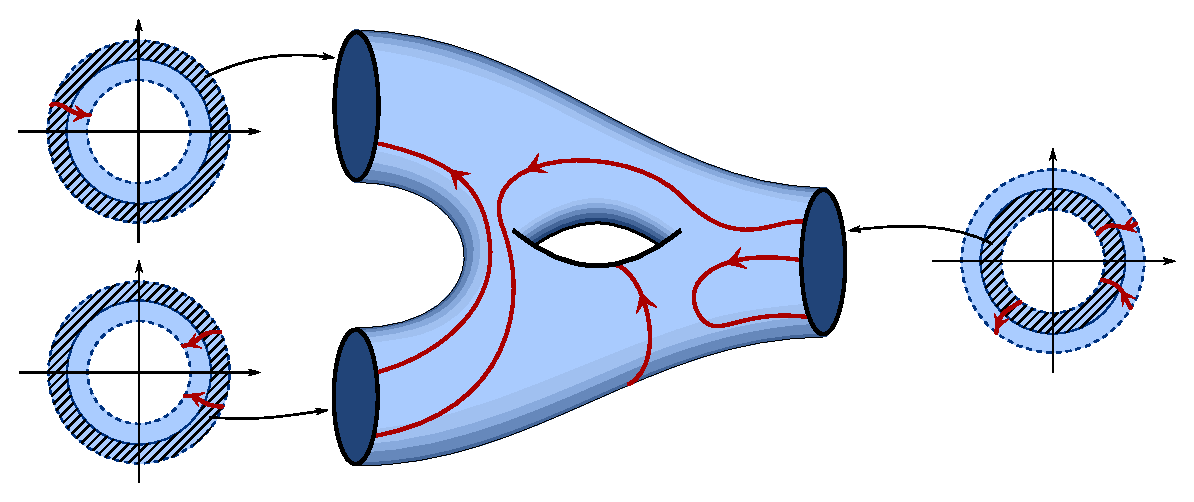
\includegraphics{pic02.eps}}}
  \put(0,0){
     \setlength{\unitlength}{.55pt}\put(-22,-8){
%     \put(136,224)   {$ \phi_\text{in} $}
%     \put(140, 22)   {$ \phi_\text{in} $}
%     \put(433,142)   {$ \phi_\text{out} $}
	 \put(295,85)   {$ Y $}
	 \put(240,190)   {$ X $}
     \put(510,180)   {$ O_{3} $}
     \put( 10,230)   {$ O_{1} $}
     \put( 10,110)   {$ O_{2} $}
     }\setlength{\unitlength}{1pt}}
  \end{picture}}
$$
\caption{A world-sheet $M$ with defect lines from $\,(O_1,O_2)\,$ to
$\,(O_{3})$.\ The two-dimensional regions of the world-sheet are all labelled with the same potential $W(x)$, while $X,Y$ are matrix factorisations of $W(x) - W(x')$. The labels on the other defect lines are omitted.}
\label{fig:wsh-defect}
\end{figure}

Consider the example shown in Figure \ref{fig:wsh-defect}, where $\cat{B} = \LG$, the two-dimensional regions are all labelled with a single potential $W(x)$ and $X,Y: W \lto W$ are $1$-morphisms. The value of $\mathcal{Z}$ on $M$ is a $\nC$-linear map
\be\label{eq:value_of_bordism}
\mathcal{Z}(M): \mathcal{Z}(O_1) \otimes \mathcal{Z}(O_2) \lto \mathcal{Z}(O_3)\,.
\ee
We would like to discuss an additional property of the physicist's Landau-Ginzburg model which is not encoded into the data of the functor $\mathcal{Z}$. Namely, it is a consequence of the way the defect conditions $X,Y$ enter the partition function \cite[(3.16)]{laz} that the vector spaces $\mathcal{Z}(O_i)$ and linear map $\mathcal{Z}(M)$ should depend continuously on the coefficients defining $Y,X$. To represent this mathematically we might try to present $\mathcal{Z}(O_i)$ as a vector bundle over a scheme $\mathscr{M}_Y \times \mathscr{M}_X$ parametrising possible labels and $\mathcal{Z}(M)$ as a morphism of these vector bundles. But there are some obstacles.
% \cite[(2.9)]{dkr1107.0495} 

Consider the incoming circle $O_2$ with its labels $Y,X$. The construction gives
\be\label{eq:zo2orig}
\mathcal{Z}(O_2) := H^0 \Hom_{\nC[x,x']}( Y, X )
\ee
which is the vector space of $2$-morphisms $Y \lto X$ in $\LG(W,W)$. Now suppose that the defect conditions are made to depend on parameters 
\[
Y = Y(t_1,\ldots,t_r)\,, \qquad X = X(u_1,\ldots,u_s)
\]
which satisfy their own equations and cut out a parametrising scheme $\mathscr{M}_Y \times \mathscr{M}_X \subseteq \mathbb{A}^{r+s}$. The question is: what kind of global object $\mathcal{Z}(O_2)$ on $\mathscr{M}_Y \times \mathscr{M}_X$ is formed by the finite-dimensional vector spaces
\[
\mathcal{Z}(O_2)_{P,Q} := H^0 \Hom_{\nC[x,x']}( Y(P), X(Q) )
\]
as $P$ varies over $\mathscr{M}_Y$ and $Q$ over $\mathscr{M}_X$? The problem is that \emph{a priori} we have
\be\label{eq:cohom_sucks}
\big\{ H^* \Hom_{\nC[x,x',t,u]}( Y(t), X(u) ) \big\}_{P,Q} \neq H^* \Hom_{\nC[x,x']}( Y(P), X(Q) )\,.
\ee
%This is a particular case of a general phenomenon: any complex of $\nC$-vector spaces $C$ is isomorphic in the derived category $\mathbb{D}(\nC)$ to $\bigoplus_n H^n(C)[n]$, but over a general ring, for instance the coordinate ring of $\mathscr{M}_Y \times \mathscr{M}_X$, this is not the case. 
The solution is to work instead with the full complex, which suggests the definition\footnote{Note that it is not enough to take the derived category of coherent sheaves, because the Hom complex is made up of non-finitely-generated modules over $\mathscr{M}_Y \times \mathscr{M}_X$.}
\be\label{eq:wuhe20}
\mathcal{Z}(O_2) := \Hom_{\nC[x,x',t,u]}( Y(t), X(u) ) \in \mathbb{D}( \operatorname{qcoh} \mathscr{M}_Y \times \mathscr{M}_X )\,.
\ee
An alternative (and we believe simpler) approach is to take $\cat{L}$ rather than $\LG$ as the input to the definition of the TFT. Before doing so, let us observe that in the situation where $X,Y$ do not depend on parameters, we may equivalently\footnote{This definition is not quite equivalent, because the displayed composite produces a complex of vector spaces quasi-isomorphic to $H^* \Hom(Y,X)$ rather than $H^0 \Hom(Y,X)$, but this is not important here.} define $\mathcal{Z}(O_2)$ to be the following composite in $\LG$:
\be\label{eq:composite_intro_o2}
\xymatrix@C+2pc{
0 \ar[r]^-X & W(x) - W(x') \ar[r]^-{Y^{\vee}} & 0
}\,.
\ee
Now let $\mathcal{Z}'$ be the TFT defined using the bicategory $\cat{L}$ as input. Then $\mathcal{Z}'(O_2)$ may likewise be computed by the composite \eqref{eq:composite_intro_o2} in $\cat{L}$, which is a $\nZ_2$-graded complex of vector spaces $Y^{\vee} \l X$ equipped with the action of a Clifford algebra. If $Y(t), X(u)$ are allowed to depend on parameters, the cut becomes a vector bundle
\be\label{eq:orynx}
\mathcal{Z}'(O_2) := Y^{\vee}(t) \l X(u)
\ee
over $\mathscr{M}_Y \times \mathscr{M}_X$ equipped with a differential and compatible Clifford action, such that
\be
\{ Y^{\vee}(t) \l X(u) \}_{P,Q} \cong Y^{\vee}(P) \l X(Q)
\ee
for every point $(P,Q)$.

Since $\cat{L}$ and $\LG$ are equivalent, the two ways \eqref{eq:wuhe20},\eqref{eq:orynx} of reading the composite \eqref{eq:composite_intro_o2} must contain the same information. However, the fact that $\eqref{eq:orynx}$ is a finite rank vector bundle over $\mathscr{M}_Y \times \mathscr{M}_X$ while \eqref{eq:wuhe20} is a complex of (non-finitely generated) quasi-coherent sheaves explains why $\cat{L}$ is better suited to this kind of problem.

%We leave the details to the aforementioned sequel \cite{??}, but here is a simple example which already shows the nontriviality of viewing correlators as functionals of the moduli of the labels on defects. Consider the following bordism which is a morphism from the empty manifold $\emptyset$ to $O$, where $X$ denotes a matrix factorisation of $V(y) - W(x)$. The value of this diagram is an element
%\[
%\mathcal{Z}(M) \in \mathcal{Z}(O) \cong Jac(V)
%\]
%By virtue of the above discussion, we may think of $\mathcal{Z}(M)$ as a \emph{section} of the trivial vector bundle with fiber $Jac(V)$ over the scheme $\mathscr{M}(W,V)$ which parametrises $1$-morphisms from $W$ to $V$ in $\LG$. If this section is not identically zero, then $V$ is called a \emph{generalised orbifold} of $W$ \cite{??} and it is of great interest to know when this is the case. From what we have said, it is clear that this is essentially a question of the geometry of $\mathscr{M}(W,V)$.

\subsubsection{Semantics of logic}

In forthcoming work we use the results of this paper to define a novel semantics of linear logic, in which formulas are interpreted by tuples $(\md{X}, \nC[x], W)$ where $\md{X}$ is a scheme and $W \in \nC[x]$ is a potential. Proofs in the logic are interpreted by certain correspondences between these pairs. To explain briefly why we are forced to use $\cat{L}$ rather than $\LG$, it is enough to describe the denotation of the Church numeral $\underline{2}$ (see \cite{murfet_ll}).

Let $x$ be a variable of the logic and suppose it has denotation $\llbracket x \rrbracket = (\Spec(\nC), \nC[x], W)$ in the semantics. Let $\mathscr{M} = \mathscr{M}(W,W)$ be the affine scheme parametrising $1$-morphisms $X: W \lto W$ in $\cat{L}$, as discussed above. Then
\begin{gather*}
\llbracket x \multimap x \rrbracket = \big(\Spec(\nC), \nC[x,x'], W(x) - W(x') \big)\,,\\
\llbracket {!}( x \multimap x ) \rrbracket = \big( \mathscr{M}, \nC, 0 \big)\,.
\end{gather*}
The proof $\underline{2}$ of the sequent ${!}(x \multimap x) \vdash x \multimap x$ is roughly speaking a bundle $\llbracket \underline{2} \rrbracket$ over the scheme $\mathscr{M}$ whose fiber over a loop $X$ is the square $X \l X$. More precisely, the denotation is the vector bundle over $\mathscr{M} \times \Spec(\nC[x,x'])$ whose fiber over a point $(X, a)$ is
\be\label{eq:bundledifferentialcliffordproof}
\llbracket \underline{2} \rrbracket_{X,a} = \left( X \l X \right) \otimes_{\nC[x,x']} \nC(a)\,.
\ee
For these definitions to work, it is necessary to be able to compute the coefficients of $X \l X$ as a function of the coefficients of $X$, so we must use $\cat{L}$ in place of $\LG$.

\medskip

\emph{Acknowledgements.} Thanks to Nils Carqueville for helpful comments on the draft, and to Ingo Runkel and Rafal Suszek for kindly providing Figure \ref{fig:wsh-defect}. %Although the sequel on linear logic is the proper place to fully acknowledge the debt, we cannot neglect to mention the important role that the beautiful ideas in Girard's geometry of interaction program \cite{girard_towards} had in shaping the present work.

\section{Background}\label{section:background}

Throughout $k$ is a commutative $\mathbb{Q}$-algebra. By default categories and functors are $k$-linear.

\subsection{Supercategories}

A superbicategory has for every $1$-morphism $F$ an associated $1$-morphism $\Psi F$ with $\Psi^2 \cong 1$, and in this sense the categories of $1$-morphisms are $\mathbb{Z}_2$-graded. The bicategory of Landau-Ginzburg models is an example of a superbicategory. Since Clifford algebras (which are $\mathbb{Z}_2$-graded) play a fundamental role in the definition of cut systems, superbicategories are the natural language. Our main references for the foundations are \cite{ellis_lauda,kang,kang2}, but we give the full definitions below as these references work only with strict bicategories.

\begin{definition} A \emph{supercategory} is a category $\cat{C}$ together with a functor $\Psi: \cat{C} \lto \cat{C}$ and a natural isomorphism $\xi: \Psi^2 \lto 1_{\cat{C}}$ satisfying the condition
\[
\xi * 1_{\Psi} = 1_{\Psi} * \xi
\]
as natural transformations $\Psi^3 \lto \Psi$. A \emph{superfunctor} $(F, \gamma)$ from a supercategory $(\cat{C}, \Psi_{\cat{C}})$ to a supercategory $(\cat{D}, \Psi_{\cat{D}})$ is a functor $F: \cat{C} \lto \cat{D}$ together with a natural isomorphism $\gamma: F \Psi_{\cat{C}} \lto \Psi_{\cat{D}} F$ satisfying
\[
1_F * \xi = (\xi * 1_F ) ( 1_{\Psi} * \gamma ) ( \gamma * 1_{\Psi} )\,.
\]
A \emph{supernatural transformation} $\varphi: F \lto G$ between superfunctors $(F,\gamma_F), (G,\gamma_G)$ is a natural transformation making the following diagram commute:
\[
\xymatrix{
F \Psi \ar[r]^-{\varphi \Psi}\ar[d]_-{\gamma_F} & G \Psi \ar[d]^-{\gamma_G}\\
\Psi F \ar[r]_-{\Psi \varphi} & \Psi G
}\,.
\] 
\end{definition}

\begin{example}\label{example:Aassup} If $A$ is a $\mathbb{Z}_2$-graded $k$-algebra there is a supercategory $\cat{A}$ with set of objects $|\cat{A}| = \mathbb{Z}_2$ and morphisms $\cat{A}(0,0) = \cat{A}(1,1) = A_0, \cat{A}(0,1) = \cat{A}(1,0) = A_1$ with the obvious composition and addition rules. The functor $\Psi$ is defined on objects by $\Psi(i) = i+1$ and on morphisms by the identity, while $\xi = 1$.
\end{example}

Let $\cat{C}$ be a supercategory. For objects $X,Y \in \cat{C}$ we define the $\mathbb{Z}_2$-graded $k$-module
\[
\cat{C}^*(X,Y) = \prod_{i \in \mathbb{Z}_2} \cat{C}(X, \Psi^i Y)\,.
\]
There is for any triple $X,Y,Z$ of objects a morphism of graded modules
\[
\cat{C}^*(Y,Z) \otimes_k \cat{C}^*(X, Y) \lto \cat{C}^*(X,Z)
\]
given for instance by $\varphi \otimes \psi \mapsto \xi \Psi( \varphi ) \psi$ when $\varphi, \psi$ are both of degree one. This makes $\cat{C}$ into a category enriched over the monoidal category of $\mathbb{Z}_2$-graded $k$-modules.

There are isomorphisms of graded modules $\cat{C}^*(X, \Psi Y) \cong \Psi \cat{C}^*(X, Y) \cong \cat{C}^*(\Psi X, Y)$ where $\Psi V = V [1]$ denotes the grading shift on a $\mathbb{Z}_2$-graded $k$-module. For $\mathbb{Z}_2$-graded $k$-modules $V,W$ we write $\Hom^0_k(V, W)$ for the module of degree zero maps and $\Hom_k^*(V, W)$ for the $\mathbb{Z}_2$-graded module of homogeneous maps. If $A$ is a $\mathbb{Z}_2$-graded $k$-algebra then $A^{\operatorname{op}}$ denotes the same underlying graded module with multiplication $f * g = (-1)^{|f||g|} gf$.

\begin{definition} Let $A$ be a $\mathbb{Z}_2$-graded $k$-algebra and $\cat{C}$ a supercategory. A \emph{left $A$-module in $\cat{C}$} is an object $X \in \cat{C}$ together with a morphism of $\mathbb{Z}_2$-graded algebras $A \lto \cat{C}^*(X,X)$. A \emph{morphism} of left $A$-modules is a morphism in $\cat{C}$ which commutes with the $A$-action in the obvious sense. The category of left $A$-modules in $\cat{C}$ is denoted $\cat{C}_A$. Right modules are defined similarly, using $A^{\operatorname{op}}$.
\end{definition}

\begin{remark}\label{remark:supercat_idempcomp} Viewing $A$ as a supercategory $\cat{A}$ as in Example \ref{example:Aassup}, there is an equivalence between the category of $A$-modules in $\cat{C}$ and the category of superfunctors $\cat{A} \lto \cat{C}$ and supernatural transformations.
\end{remark}

\begin{remark}\label{remark:idempotent_completion} The \emph{idempotent completion} $\cat{C}^\omega$ of a category $\cat{C}$ has as objects pairs $(X,e)$ consisting of an object $X \in \cat{C}$ and an idempotent endomorphism $e: X \lto X$. In $\cat{C}^\omega$ a morphism $\phi: (X,e) \lto (Y,e)$ is a morphism $\phi: X \lto Y$ satisfying $\phi e = \phi$ and $e \phi = \phi$. The identity on $(X,e)$ is $e$. There is a fully faithful functor $\iota: \cat{C} \lto \cat{C}^{\omega}, \iota(X) = (X,1_X)$ which is an equivalence if $\cat{C}$ is idempotent complete (i.e. all idempotents split in $\cat{C}$).

If $\cat{C}$ is a supercategory then there is a functor $\Psi^\omega: \cat{C}^\omega \lto \cat{C}^\omega$ defined on objects by $\Psi(X,e) = (\Psi X, \Psi e)$ and a natural isomorphism $\xi: \Psi^\omega \circ \Psi^\omega \lto 1_{\cat{C}^\omega}$ defined by $\xi_{(X,e)} = e \xi_X$. The tuple $(\cat{C}^\omega, \Psi^\omega, \xi^\omega)$ is a supercategory.
\end{remark}

For background on bicategories see \cite{bor94} and the references in \cite{lgdual}. We follow the notation of \cite{lgdual}, so that lower case letters $a,b, \ldots$ denote objects of a bicategory, while upper case letters $X,Y, \ldots$ and greek letters $\alpha, \beta, \ldots$ respectively denote $1$-morphisms and $2$-morphisms. Units are denoted $\Delta$, associators are $\alpha$, and unitors are $\lambda, \rho$. The composition of $Y,X$ is denoted $YX$ or $Y \circ X$.

\begin{definition} A \emph{superbicategory} is a bicategory $\cat{B}$ together with the data:
\begin{itemize}
\item For each object $a$ a $1$-morphism $\Psi_a: a \lto a$ and a $2$-isomorphism $\xi_a: \Psi^2_a \lto \Delta_a$.
\item For each $1$-morphism $X: a \lto b$ a natural $2$-isomorphism $\gamma_X: X \Psi_a \lto \Psi_b X$.
\end{itemize}
This data is required to satisfy the following axioms:
\begin{itemize}
\item For each composable pair $X,Y$ of $1$-morphisms the diagram
\[
\xymatrix@C+2pc@R+1pc{
(YX) \Psi \ar[rrr]^-{\gamma_{YX}} \ar[d]_-{\alpha} & & & \Psi ( YX )\\
Y ( X \Psi ) \ar[r]_-{1_Y * \gamma_X} & Y( \Psi X ) \ar[r]_-{\alpha^{-1}} & ( Y \Psi ) X \ar[r]_-{\gamma_Y * 1_X} & (\Psi Y ) X \ar[u]_-{\alpha}
}
\]
commutes.
\item For every object $a$, $\xi_a * 1_\Psi = 1_\Psi * \xi_a$.
\item For every $1$-morphism $X : a \lto b$, $1_X * \xi_a = ( \xi_b * 1_X ) ( 1_\Psi * \gamma_X ) (\gamma_X * 1_\Psi )$.
\end{itemize}
\end{definition}

\begin{example} Supercategories, superfunctors and supernatural transformations form a superbicategory $\Cat^{\operatorname{sup}}_k$.
\end{example}

A superbicategory can be constructed out of a bicategory $\cat{B}$ in which the categories $\cat{B}(a,b)$ are all equipped with the structure of supercategories; see Appendix \ref{section:constructing_superbicategories}.

\begin{example}\label{example:bicategory_m} There is a bicategory of $\mathbb{Z}_2$-graded $k$-algebras where $1$-morphisms are $\mathbb{Z}_2$-graded bimodules and $2$-morphisms are degree zero bimodule maps. Given a $B$-$A$-module $M$ the shift $M[1]$ has the grading $M[1]_i = M_{i+1}$ and the left and right action given by
\[
b \cdot m = (-1)^{|b|} bm, \qquad m \cdot a = (-1)^{|a|} m a\,.
\]
This is a functor $\Psi = (-)[1]$ on the category of $B$-$A$-bimodules and with $\xi = 1$ this defines the structure of a supercategory on this category of bimodules. The usual isomorphisms of bimodules $\tau$
\begin{align}
N[1] \otimes M &\lto (N \otimes M)[1], \qquad n \otimes m \mapsto n \otimes m \label{eq:shift_iso_a}\\
N \otimes M[1] &\lto (N \otimes M)[1], \qquad n \otimes m \mapsto (-1)^{|n|} n \otimes m\label{eq:shift_iso_b}
\end{align}
satisfy the conditions in Appendix \ref{section:constructing_superbicategories} and therefore give the bicategory of $\mathbb{Z}_2$-graded algebras and bimodules the structure of a superbicategory.
\end{example}

\begin{definition} Given two superbicategories $\cat{B}, \cat{C}$ a \emph{lax superfunctor} $\Phi: \cat{B} \lto \cat{C}$ is a lax functor together with, for each object $a$ in $\cat{B}$, a $2$-morphism
\[
\kappa_a: \Psi_{\Phi a} \lto \Phi( \Psi_a )
\]
satisfying two coherence conditions:
\begin{itemize}
\item[(a)] for all $a$, commutativity of
\[
\xymatrix@C+2pc{
\Psi_{\Phi a} \Psi_{\Phi a} \ar[dd]_-{\xi}\ar[r]^-{\kappa * \kappa} & \Phi( \Psi_a ) \Phi( \Psi_a ) \ar[d]\\
& \Phi( \Psi_a \Psi_a ) \ar[d]^-{\Phi(\xi)}\\
\Delta_{\Phi a} \ar[r] & \Phi( \Delta_a )
}
\]
\item[(b)] for each $1$-morphism $X: a \lto b$ in $\cat{B}$, commutativity of
\[
\xymatrix@C+2pc{
\Phi(X) \Psi_{\Phi a} \ar[d]_-{\gamma} \ar[r]^-{1 * \kappa} & \Phi(X) \Phi(\Psi_a) \ar[r] & \Phi( X \Psi_a ) \ar[d]^-{\Phi(\gamma)}\\
\Psi_{\Phi b} \Phi(X) \ar[r]_-{\kappa * 1} & \Phi(\Psi_b) \Phi(X) \ar[r] & \Phi( \Psi_b X)
}
\]
\end{itemize}
A \emph{strong superfunctor} is a lax superfunctor with $\kappa_a$ an isomorphism for every object $a$.
\end{definition}

\subsection{The superbicategory of Landau-Ginzburg models}\label{section:superbicatLG}

A polynomial $W \in k[x_1,\ldots,x_n]$ is a \emph{potential} if it satisfies the three conditions set out in \cite[Section 2.2]{lgdual}, the two most important being that the partial derivatives $\partial_{x_1} W, \ldots, \partial_{x_n} W$ form a quasi-regular sequence in $k[x]$ and that the quotient $J_W = k[x]/(\partial_{x_1} W, \ldots, \partial_{x_n} W)$ is a finitely generated free $k$-module. Typical examples are the ADE singularities \cite[I \S 2.4]{greuel} of which the simplest are the $A_N$-singularities $W_{A_N} = x_1^{N+1} + x_2^2 + \cdots + x_n^2$ .

A \emph{matrix factorisation} of $W$ over $k[x]$ is a $\mathbb{Z}_2$-graded free $k[x]$-module $X = X^0 \oplus X^1$ together with an odd operator (the differential) $d_X: X \lto X$ satisfying $d_X^2 = W \cdot 1_X$. A matrix factorisation $(X,d_X)$ is \emph{finite rank} if the underlying free module is finitely generated. In this case we may, after choosing a homogeneous basis, write
\[
d_X = \begin{pmatrix} 0 & d_X^1 \\ d_X^0 & 0 \end{pmatrix}
\]
for matrices of polynomials $d_X^0, d_X^1$. Morphisms of matrix factorisations are degree zero $k[x]$-linear maps which commute with the differentials. There is a homotopy relation on morphisms, and the \emph{homotopy category} $\HMF(k[x],W)$ of matrix factorisations has as objects matrix factorisations and as morphisms the equivalence classes of morphisms of matrix factorisations up to homotopy. By $\hmf(k[x],W)$ we denote the full subcategory of finite rank matrix factorisations. For background we refer to \cite{yoshino98}.

By $\hmf(k[x],W)^{\oplus}$ we denote the full subcategory of $\HMF(k[x],W)$ consisting of matrix factorisations which are direct summands (in the homotopy category) of finite rank matrix factorisations. Since $\HMF(k[x],W)$ is idempotent complete, there is an equivalence (see Remark \ref{remark:idempotent_completion} for the notation)
\be\label{eq:omegavsoplus}
\hmf(k[x],W)^\omega \lto \hmf(k[x],W)^{\oplus}
\ee
sending a pair $(X,e)$ to an infinite rank matrix factorisation splitting the idempotent $e$.

If $(X,d_X)$ is a matrix factorisation then so is $(X[1], -d_X)$, and this defines a functor $\Psi = (-)[1]$ on the homotopy category of matrix factorisations. Together with the identity $\xi: \Psi^2 \lto 1$ this makes $\HMF(k[x],W)$ and $\hmf(k[x],W)$ into supercategories.

The bicategory of Landau-Ginzburg models $\LG$ has for its objects pairs $(x,W)$ consisting of an ordered set of variables $x = (x_1,\ldots,x_n)$ and a potential $W \in k[x] = k[x_1,\ldots,x_n]$. Given potentials $W \in k[x]$ and $V \in k[y]$ the supercategory $\cat{LG}(W,V)$ is
\[
\cat{LG}(W,V) = \hmf(k[x,y], V - W)^{\oplus}\,.
\]
Given a third potential $U \in k[z]$ the composition law is a functor
\[
\LG(W,V) \otimes_k \LG(V, U) \lto \LG(W, U)
\]
which sends a pair of $1$-morphisms $X: W \lto V$ and $Y: V \lto U$ to the tensor product
\begin{equation}\label{eq:tensor_comp}
Y \otimes X = ( Y \otimes_{k[y]} X, d_{Y \otimes X} = d_Y \otimes 1 + 1 \otimes d_X )\,.
\end{equation}
This statement requires some care: $k[x,y,z]$ is an infinite rank free module over $k[x,z]$ and so $Y \otimes X$ is an infinite rank matrix factorisation of $U - W$ over $k[x,z]$. However one can prove that $Y \otimes X$ is a direct summand of a finite rank matrix factorisation \cite{dm1102.2957} and therefore a valid object in $\LG(W,U)$.

Let $W \in k[x_1,\ldots,x_n]$ be a potential and $W(x')$ the same polynomial but in a second set of variables $x_1',\ldots,x_n'$. Using formal symbols $\Theta_i$ of odd degree, we define the $k[x,x']$-module
\[
\Delta_W = \bigwedge \big( \bigoplus_{i=1}^n k[x,x'] \cdot \Theta_i \big)\,.
\]
Equipped with a certain differential (see \cite{lgdual}) this is a matrix factorisation of $W(x) - W(x')$ and defines the unit in $\cat{LG}(W,W)$ for composition of $1$-morphisms. For the associator and unitor maps $\rho: X \otimes \Delta_W \lto X$ and $\lambda: \Delta_V \otimes X \lto X$ we also refer to \emph{ibid.}

\begin{lemma} $\LG$ is a superbicategory.
\end{lemma}
\begin{proof}
The categories $\LG(W,V)$ are all naturally supercategories, and the same isomorphisms as in \eqref{eq:shift_iso_a}, \eqref{eq:shift_iso_b} define the necessary natural isomorphisms $\tau$ to equip $\LG$ with the structure of a superbicategory with $\Psi_W = \Delta_W[1]$, using Appendix \ref{section:constructing_superbicategories}.
\end{proof}

The superbicategory structure on $\LG$ is used implicitly in \cite[Section 7]{lgdual}.

\subsection{Partial derivatives as homotopies}\label{section:partial}

Let $R = k[x_1,\ldots,x_n]$ be a polynomial ring and $X$ a finite rank matrix factorisation of $W$ over $R$. Let us fix a homogeneous basis for $X$ so that we may identify $d_X$ with a matrix, and differentiate this matrix entry-wise to obtain the matrix $\lambda_i = \partial_{x_i}(d_X)$. It is easy to check that

\begin{lemma}\label{lemma:homotopy_indept} The odd $R$-linear operator $\lambda_i$ on $X$ is independent, up to homotopy, of the choice of basis.
\end{lemma}

\begin{lemma} As operators on $X$ we have $[ d_X, \lambda_i ] = \partial_{x_i} W \cdot 1_X$.
\end{lemma}
\begin{proof}
Applying the Leibniz rule to the equation $d_X d_X = W$ we obtain
\be\label{eq:partials_are_homotopies}
d_X \partial_{x_i}(d_X) + \partial_{x_i}(d_X) d_X = \partial_{x_i} W
\ee
as claimed.
\end{proof}

It follows that any element in the Jacobi ideal $( \partial_{x_1}W , \ldots, \partial_{x_n} W )$ acts null-homotopically on any morphism in the homotopy category $\hmf(R,W)$. Moreover these homotopies $\lambda_i$ are central, in the following sense:

\begin{lemma}\label{lemma:naturalityoflambda} Let $\phi: X \lto X'$ be a morphism of matrix factorisations and write $\lambda_i = \partial_{x_i}(d_X)$ and $\lambda'_i = \partial_{x_i}(d_{X'})$. There is a homotopy $\phi \lambda_i \simeq \lambda'_i \phi$.
\end{lemma}
\begin{proof}
From $d_{X'} \phi = \phi d_X$ we deduce
\[
\partial_{x_i}( d_{X'} ) \phi + d_{X'} \partial_{x_i}( \phi ) = \partial_{x_i}( \phi ) d_X + \phi \partial_{x_i}( d_X )
\]
and hence
\[
\partial_{x_i}( d_{X'} ) \phi - \phi \partial_{x_i}( d_X ) = \partial_{x_i}(\phi) d_X - d_{X'} \partial_{x_i}(\phi)
\]
as claimed.
\end{proof}

\begin{lemma}\label{lemma:commutator_of_lambdas} There is a homotopy $[ \lambda_i, \lambda_j ] \simeq \partial_{x_i x_j}(W) \cdot 1_X$.
\end{lemma}
\begin{proof}
Differentiating \eqref{eq:partials_are_homotopies} with respect to $j$ leaves
\[
\partial_{x_j}(d_X) \partial_{x_i}(d_X) + d_X \partial_{x_jx_i}(d_X) + \partial_{x_jx_i}(d_X) d_X + \partial_{x_i}(d_X) \partial_{x_j}(d_X) = \partial_{x_ix_j}W
\]
from which we read off
\[
\lambda_i \lambda_j + \lambda_j \lambda_i = \partial_{x_ix_j}W + [d, -\partial_{x_jx_i}(d_X)]\,.
\]
\end{proof}

\subsection{Clifford algebras}\label{section:clifford_algs}

The cut operation in $\cat{L}$ produces objects which are representations of Clifford algebras. We briefly recall the basic theory of these algebras and their modules; for a full discussion see \cite{friedrich}. For $n \ge 0$ the Clifford algebra $C_n$ is the associative $\mathbb{Z}_2$-graded $k$-algebra generated by odd elements $\gamma_1,\ldots,\gamma_n$ and $\gamma_1^\dagger, \ldots, \gamma_n^\dagger$ subject to the following relations
\be\label{eq:clifford_relations}
[\gamma_i, \gamma_j] = 0, \qquad [\gamma_i^\dagger, \gamma_j^\dagger] = 0, \qquad [\gamma_i, \gamma_j^\dagger] = \delta_{ij}\,.
\ee
for all $1 \le i, j \le n$. In this paper all our commutators are graded, $[a,b] = ab - (-1)^{|a||b|} ba$. We set $C_0 = k$. These Clifford algebras have essentially only one nontrivial representation, sometimes called the \emph{spinor representation} \cite[p.14]{friedrich}. To define this representation we use the $\nZ_2$-graded $k$-module
\[
F_n = k \theta_1 \oplus \cdots \oplus k \theta_n
\]
where the $\theta_i$ are formal variables of odd degree, and set
\be
S_n = \bigwedge F_n = \bigwedge\big( k \theta_1 \oplus \cdots \oplus k \theta_n \big)\,.
\ee

\begin{definition}\label{defn:contraction} Left multiplication in the exterior algebra defines an odd operator
\begin{gather*}
\theta_i \wedge (-): S_n \lto S_n\,,\\
\theta_{j_1} \cdots \theta_{j_r} \mapsto \theta_i \theta_{j_1} \cdots \theta_{j_r}\,.
\end{gather*}
Contraction from the left defines an odd operator
\begin{gather*}
\theta_i^*\, \lrcorner\, (-): S_n \lto S_n\,,\\
\theta_{j_1} \cdots \theta_{j_r} \mapsto \sum_{l=1}^r (-1)^{(l-1)} \delta_{i,j_l} \theta_{j_1} \cdots \widehat{ \theta_{j_l} } \cdots \theta_{j_r}\,.
\end{gather*}
\end{definition}

Usually we write simply $\theta_i$ for the operator $\theta_i \wedge (-)$ and $\theta_i^*$ for the operator $\theta_i^*\, \lrcorner\, (-)$. The spinor representation is defined by the next lemma, which also shows that the algebras $C_n$ are Morita trivial in the sense that they are isomorphic to the endomorphism algebras of a finite rank free $\mathbb{Z}_2$-graded $k$-module.

\begin{lemma}\label{defn:spinorrep} The map $C_n \lto \End_k(S_n)$ defined by
\[
\gamma_i \mapsto \theta_i \wedge (-), \qquad \gamma_i^\dagger \mapsto \theta_i^*\, \lrcorner\, (-)
\]
is an isomorphism of $\mathbb{Z}_2$-graded $k$-algebras.
\end{lemma}

In particular this means that every $\mathbb{Z}_2$-graded $C_n$-module is isomorphic to $S_n \otimes_k V$ for some $\mathbb{Z}_2$-graded $k$-module $V$. Using the isomorphism of $k$-modules
\[
F_m \oplus F_n \cong F_{m+n}
\]
which maps the ordered basis $\theta_1,\ldots,\theta_m$ of $F_m$ to the first $m$ basis elements of $F_{m+n}$ in their given order, and the ordered basis of $F_n$ to the last $n$ basis elements, we define
\[
S_m \otimes_k S_n = \bigwedge F_m \otimes_k \bigwedge F_n \cong \bigwedge F_{m+n} = S_{m+n}\,.
\]
From this we deduce an isomorphism of algebras
\begin{equation}\label{eq:algebra_A_additive}
C_m \otimes_k C_n \cong C_{m+n}\,.
\end{equation}
Given $m, n \ge 0$ we introduce notation for the $C_m$-$C_n$-bimodule
\begin{equation}
S_{m,n} = S_m \otimes_k S_n^* \cong \Hom_k(S_n,S_m)
\end{equation}
where $S_n^* = \Hom_k(S_n, k)$. There is an isomorphism of $C_l$-$C_n$-bimodules
\begin{equation}\label{eq:isosbimodule}
S_{l,m} \otimes_{C_m} S_{m,n} = S_l \otimes_k S_m^* \otimes_{C_m} S_m \otimes_k S_n^* \cong S_{l,n}\,.
\end{equation}

\begin{definition}\label{defn:idempotent_e} For $n \ge 0$ let $e_n \in C_n$ denote the element
\[
e_n = \gamma_1^\dagger \cdots \gamma_n^\dagger \gamma_n \cdots \gamma_1\,.
\]
This is the idempotent corresponding to the summand $k \cdot 1$ of $S_n$.
\end{definition}

\begin{definition}\label{defn:idempotent_gen} More generally, given $m, n \ge 0$ consider the $k$-linear map
\[
\xymatrix{
S_n \ar[r] & k \cdot 1 \ar[r]^{\operatorname{inc}} & S_m
}
\]
given by the projection to $k \cdot 1$ followed by the inclusion into $S_m$. This defines an element
\[
\iota_{m,n} \in \Hom_k(S_n, S_m) = S_m \otimes_k S_n^*\,.
\]
Then obviously $\iota_{n,n} = e_n$.
\end{definition}

\begin{remark} Recall that given a finite rank free $k$-module $V$ and a symmetric bilinear form $B: V \otimes_k V \lto k$ the associated Clifford algebra $\operatorname{Cl}(V, B)$ is the associative $k$-algebra generated by the elements of $V$ subject to the relations
\[
vw + wv = B(v,w) \cdot 1\,.
\]
This is a $\mathbb{Z}_2$-graded $k$-algebra when we assign $|v| = 1$ for all $v \in V$ and $|1| = 0$. If we take $V = F \oplus F^*$ with the bilinear form $B$ under which $B(F,F) = 0, B(F^*, F^*) = 0$ and for $x \in F$ and $\nu \in F^*$, $B(x, \nu) = \frac{1}{2} \nu(x)$, then $C_n$ is the Clifford algebra of the pair $(V,B)$.
\end{remark}

\section{The Clifford thickening}\label{section:cliff_thick}

Let $\cat{T}$ be a small idempotent complete supercategory. We construct a new supercategory $\cat{T}^\bullet$ called the \emph{Clifford thickening} in which the objects are pairs $(X,n)$ of an integer $n \ge 0$ and a left $C_n$-module $X$ in $\cat{T}$. Recall that if $A$ is a $\mathbb{Z}_2$-graded $k$-algebra then $\cat{T}_A$ denotes the supercategory of $A$-modules in $\cat{T}$ with $A$-linear maps.

%The upshot is that if $A$ is a Morita trivial $\mathbb{Z}_2$-graded $k$-algebra and if $X \in \cat{T}$ is a left $A$-module, while $V$ is a $\mathbb{Z}_2$-graded right $A$-module (in the usual sense, i.e. in the category of $k$-modules) then there is an object $V \otimes_A X$ in $\cat{T}$ which is functorial in both $V$ and $X$. Morever if $V$ is a $B$-$A$-bimodule then $V \otimes_A X$ is naturally a left $B$-module, and so on. 

Similarly to Example \ref{example:bicategory_m} there is a superbicategory $\cat{M}$ of Morita trivial $\mathbb{Z}_2$-graded $k$-algebras: $1$-morphisms are $\mathbb{Z}_2$-graded bimodules which are finitely generated and projective over $k$ and $2$-morphisms are degree zero bimodule maps. We will need the operation of tensoring objects of $\cat{T}$ with $k$-modules, which is recalled in Appendix \ref{section:tensorproduct_supcat}. 

\begin{proposition} The assignment of the supercategory $\cat{T}_A$ to an algebra $A$ and of the superfunctor $\Phi_V = V \otimes_A (-)$ to a $B$-$A$-bimodule $V$ determines a strong superfunctor
\[
\Phi^{\cat{T}}: \cat{M} \lto \Cat^{\operatorname{sup}}_k
\]
to the superbicategory of small supercategories and superfunctors.
\end{proposition}
\begin{proof}
The isomorphism $\Phi_W \circ \Phi_V \cong \Phi_{W \otimes V}$ is given by Lemma \ref{lemma:assoctensor}, and apart from that the only checking that needs to be done are straightforward coherence diagrams.
\end{proof}

Next we construct a strong functor into $\cat{M}$ which picks out the Clifford algebras.

\begin{definition}
Let $\mathbb{N}$ denote the category of integers $n \ge 0$ with a unique morphism $\phi_{m,n}: n \lto m$ for each pair $m,n$. %This category is monoidal with $m \otimes n = m + n$.
\end{definition}

We view $\mathbb{N}$ as a bicategory with only identity $2$-morphisms.

\begin{lemma} There is a strong functor $\mathbb{N} \lto \cat{M}$ defined by
\begin{gather*}
n \mapsto C_n = \End_k( S_n ),\\
\phi_{m,n} \mapsto S_{m,n} = S_m \otimes_k S_n^*\,.
\end{gather*}
\end{lemma}

The composite of these strong functors is a strong functor
\begin{equation}\label{eq:strongfunctorgroth}
\xymatrix@C+1pc{
\mathbb{N} \ar[r] & \cat{M} \ar[r]^-{\Phi^{\cat{T}}} & \Cat^{\operatorname{sup}}_k
}
\end{equation}
sending $n$ to the category of left $C_n$-modules in $\cat{T}$ and $\phi_{m,n}$ to the functor $S_{m,n} \otimes_{C_n} -$. There is a close connection between strong functors into the bicategory of small categories, and what are called cofibered categories, given by the Grothendieck construction \cite{vistoli}.

\begin{definition} The \emph{Clifford thickening} $\cat{T}^\bullet$ of the supercategory $\cat{T}$ is the category which results from the Grothendieck construction applied to the strong functor \eqref{eq:strongfunctorgroth}.
\end{definition}

More concretely $\cat{T}^\bullet$ is the category with objects all pairs $(X,n)$ of an integer $n \ge 0$ and an object $X \in \cat{T}$ together with a left $C_n$-action. A morphism $\alpha: (X,n) \lto (Y,m)$ is a morphism of $C_m$-modules $\alpha: S_{m,n} \otimes_{C_n} X \lto Y$. Composition of a pair of morphisms
\begin{equation}\label{eq:comp_chain0}
\xymatrix{
(X,n) \ar[r]^-{\alpha} & (Y,m) \ar[r]^-{\beta} & (Z,l)
}
\end{equation}
is given by the morphism of $C_l$-modules
\begin{equation}\label{eq:comp_chain1}
\xymatrix@C+1pc{
S_{l, n} \otimes_{C_n} X \ar[r]^-{\cong} & (S_{l,m} \otimes_{C_m} S_{m,n}) \otimes_{C_n} X \ar[d]^-{\cong}\\
& S_{l,m} \otimes_{C_m} ( S_{m,n} \otimes_{C_n} X ) \ar[r]^-{ 1 \otimes \alpha } & S_{l,m} \otimes_{C_m} Y \ar[r]^-{\beta} & Z\,.
}
\end{equation}
There is a canonical functor $p: \cat{T}^\bullet \lto \mathbb{N}$ defined by $p(X,n) = n$, which defines a cofibered category over $\mathbb{N}$ by the definition of the Grothendieck construction. This definition has the benefit of being derived from a general construction, but there is an alternative description of morphisms which is less cumbersome:

\begin{definition} Let $\cat{T}^{\star}$ be the category with the same objects as $\cat{T}^\bullet$ and
\begin{align*}
\cat{T}^{\star}( (X,n), (Y,m) ) &= \Big\{ \alpha \in \cat{T}(X,Y) \l \alpha \gamma_i = 0 \text{ for } 1 \le i \le n \text{ and }\\
&\qquad \qquad\qquad \qquad \;\; \gamma_i^\dagger \alpha = 0 \text{ for } 1 \le i \le m \Big\}\,.
\end{align*}
Composition is as in $\cat{T}$, but the identity on $(X,n)$ in $\cat{T}^\star$ is the morphism
\[
1^*_{(X,n)} = e_n
\]
where $e_n$ is the action on $X$ of the canonical idempotent from Definition \ref{defn:idempotent_e}.
\end{definition}

\begin{lemma}\label{lemma:equivcliffordthick} $\cat{T}^{\star}$ is a category and there is an equivalence of categories
\[
\Theta: \cat{T}^\bullet \lto \cat{T}^{\star}
\]
\end{lemma}
\begin{proof}
To prove that $\cat{T}^{\star}$ is a category it only needs to be checked that $1^*_{(X,n)}$ really acts as an identity. Let $\alpha: X \lto Y$ be a morphism in $\cat{T}^{\star}$ and consider
\begin{align*}
\alpha e_n &= \alpha \gamma_1^\dagger \cdots \gamma_n^\dagger \gamma_n \cdots \gamma_1\\
&= \alpha \left( \gamma_1^\dagger \cdots \gamma_{n-1}^\dagger \gamma_{n-1} \cdots \gamma_1 - \gamma_1^\dagger \cdots \gamma_n \gamma_n^\dagger \cdots \gamma_1 \right)\\
&= \alpha \gamma_1^\dagger \cdots \gamma_{n-1}^\dagger \gamma_{n-1} \cdots \gamma_1
\end{align*}
since in the second summand within the brackets, there is nothing to stop $\gamma_n$ from commuting to the left and annihilating with $\alpha$. Proceeding inductively, we see that $\alpha e_n = \alpha$. The proof that $e_n \alpha = \alpha$ is similar.

The functor $\Theta$ is defined to be the identity on objects, and given $\beta: (X,n) \lto (Y,m)$ in $\cat{T}^{\bullet}$ which is a morphism $\beta: S_{m,n} \otimes_{C_n} X \lto Y$ in $\cat{T}$ we define
\begin{gather*}
\Theta(\beta): X \lto Y\,,\\
\Theta(\beta)( x ) = \beta( \iota_{m,n} \otimes x )
\end{gather*}
where $\iota_{m,n}$ is as in Definition \ref{defn:idempotent_gen}. We relegate the proof that this functor gives a bijection on morphism sets to Lemma \ref{lemma:morphisms_two_forms}. Functoriality is easily checked, and $\Theta(1_X) = e_n$ since by definition $\iota_{n,n} = e_n$.
\end{proof}

Every $C_n$-module $X$ in $\cat{T}$ is of the form $S_n \otimes_k V$ for some object $V$. It will be important later to know exactly how to extract the object $V$ from $X$ by splitting an idempotent.

\begin{lemma}\label{lemma:whackamole} Let $X$ be a $C_n$-module in $\cat{T}$. The idempotent $e_n: X \lto X$ splits, say 
\[
\xymatrix@C+2pc{
X \ar@<1ex>[r]^-{f_0} & V \ar@<1ex>[l]^-{g_0}
}
\]
with $f_0 g_0 = 1_V$ and $g_0 f_0 = e_n$ and in $\cat{T}^\bullet$ there are mutually inverse isomorphisms
\[
\xymatrix@C+2pc{
(X, n) \ar@<1ex>[r]^-{f} & (V,0) \ar@<1ex>[l]^-{g}\,.
}
\]
induced by $f_0,g_0$. In particular
\be
S_n^* \otimes_{C_n} X \cong V\,, \qquad S_n \otimes_k V \cong X\,.
\ee
\end{lemma}
\begin{proof}
The map $f_0$ is a morphism $(X,n) \lto (V,0)$ in $\cat{T}^{\star}$ since
\[
f_0 \gamma_i = f_0 e_n \gamma_i = f_0 \gamma_1^\dagger \cdots \gamma_n^\dagger \gamma_n \cdots \gamma_1 \gamma_i = 0\,.
\]
Similarly $g_0$ defines a morphism $(V,0) \lto (X,n)$. Let $f,g$ be the morphisms in $\cat{T}^\bullet$ corresponding to $f_0,g_0$ under the equivalence of Lemma \ref{lemma:equivcliffordthick}. To prove that $fg = 1_{(X,n)}$ and $gf = 1_{(V,0)}$ in $\cat{T}^{\bullet}$ it suffices to prove that $f_0 g_0 = 1^*_{(X,n)} = e_n$ and $g_0 f_0 = 1^*_{(V,0)}$ in $\cat{T}^{\star}$. But this is true by definition.
\end{proof}

\begin{lemma}\label{lemma:embedcliffordthick} $\cat{T}^\bullet$ is a supercategory and the functor $\iota: \cat{T} \lto \cat{T}^\bullet$ defined by $\iota(X) = (X,0)$ is an equivalence of supercategories.
\end{lemma}
\begin{proof}
The supercategory structure is given by the functor $\Psi: \cat{T}^\bullet \lto \cat{T}^\bullet$ where $\Psi(X,n) = ( \Psi X, n )$ and $\Psi X$ has the $C_n$-action given by Definition \ref{defn:psimodule}. The functor $\iota$ is fully faithful and it follows from Lemma \ref{lemma:whackamole} that it is essentially surjective.
\end{proof}

%\begin{remark}\label{remark:tensor_and_idempotent} It may seem odd to labour to construct a category $\cat{C}^\bullet$ equivalent to $\cat{C}$. The point is that while $(X,n)$ and $(\widetilde{X}, 0)$ are isomorphic in $\cat{C}^\bullet$, they still represent quantitatively different states of knowledge. If $\widetilde{X}$ is known then $X$ may be easily constructed by taking direct sums, but if $X$ is known then forming the tensor product $\widetilde{X}$ is equivalent to splitting the idempotent $e_n: X \lto X$ and this requires work.
% If $X$ is an $A_n$-module in $\cat{C}$, then the defining property of $\widetilde{X} = S_n^* \otimes_{A_n} X$ is that there is a morphism $\eta: X \lto \widetilde{X}$ satisfying $\eta \circ a_i = 0$ for all $1 \le i \le n$ and which is universal with this property. That is, given any morphism $\delta:X  \lto Y$ with this property there is a unique morphism $\kappa: \widetilde{X} \lto Y$ such that $\kappa \circ \eta = \delta$. A morphism $\delta: X \lto Y$ satisfies $\delta \circ a_i = 0$ for $1 \le i \le n$ if and only if $\delta \circ ( 1 - e_n ) = 0$.

%For each $n$ the fiber of the functor $p: \cat{C}^\bullet \lto \mathbb{N}$ over $n$ is $\cat{C}_{A_n}$. We may depict the cofibered category $p$ as follows:
%\begin{equation}\label{eq:cofibered_diagram}
%\xymatrix@C+3pc@R+1pc{
%\cat{C} \ar@{.}[d] \ar@<1ex>[rrr]^-{E} & & & \cat{C}_{A_n} \ar@{.}[d] \ar@<1ex>[lll]^-{F}\\
%0 \ar@{.>}@<0.8ex>[r] & 1 \ar@{.>}@<0.8ex>[r]\ar@{.>}@<0.8ex>[l] & \cdots \ar@{.>}@<0.8ex>[l]\ar@{.>}@<0.8ex>[r] & n \ar@{.>}@<0.8ex>[l]
%}\,.
%\end{equation}
%The transport between the fibers is given by the equivalences
%\[
%E(-) = S_{n} \otimes_k (-), \qquad F(-) = S^*_{n} \otimes_{A_n} (-)\,.
%\]
%While these functors are adjoint, and therefore uniquely determine one another, we have explained that there is a fundamental asymmetry between them from the point of view of computation: knowledge of an object of $\cat{C}^\bullet$ over $n$ represents a state of higher uncertainty than knowledge of an object over $m < n$, given that in the end both objects ``only'' contain the information of the corresponding object $\widetilde{X}$ over zero, but more work is necessary to extract this information from an object of $\cat{C}_{A_n}$ than from an object of $\cat{C}_{A_m}$.
%\end{remark}

%\begin{remark}\label{remark:tensor_in_steps} Given $(X,n) \in \cat{T}^\bullet$, one way to compute the tensor product
%\[
%S_{n+1,n} \otimes_{A_n} X = (S_{n+1} \otimes_k S_n^*) \otimes_{A_n} X \cong S_{n+1} \otimes_k ( S_n^* \otimes_{A_n} X )
%\]
%is to compute $S_n^* \otimes_{A_n} X$ and then take direct sums. Alternatively,
%\begin{align*}
%S_{n+1,n} \otimes_{A_n} X &= S_{n+1} \otimes_k S_n^* \otimes_{A_n} X\\
%&\cong S_1 \otimes_k S_n \otimes_k S_n^* \otimes_{A_n} X \\
%&\cong S_1 \otimes_k A_n \otimes_{A_n} X \\
%&\cong S_1 \otimes_k X\,.
%\end{align*}
%That is, if we equip $S_1 \otimes_k X = X \oplus \Psi X$ with an $A_{n+1} \cong A_1 \otimes A_n$ action by making $A_n$ act on $X$ and $A_1$ act on $S_1$, this computes the tensor product. In a similar way, $S_{n-1,n} \otimes_{A_n} X$ is computed by splitting the idempotent $a_1^\dagger a_1$ on $X$, so that the functor $F$ of \eqref{eq:cofibered_diagram} may be computed in $n$ steps by splitting $a_1^\dagger a_1$, then $a_2^\dagger a_2$, and so on.
%\end{remark}
%TODO note: $S_{m,n} \otimes_{A_n}$ is an equivalence so all fibers are isomorphic to $\cat{C}$.

\section{The superbicategory $\cat{L}$}\label{section:lg_cut_system}

%In this section we introduce the cut system $\cat{L}$, beginning with a sketch of the major pieces and then proceeding to the technical details. The objects of the cut system are the same as the objects of the bicategory $\LG$, that is, pairs $(x, W)$ consisting of a set of variables $x = (x_1,\ldots,x_n)$ and a potential $W \in k[x]$. Such an object is often written as $W$ or $W(x)$. The integer $\pi(x,W) = n$ is the number of variables.

In this section we define a superbicategory without units $\cat{L}$. Later we will prove that this bicategory is equivalent to $\LG$, although this will not be apparent at first. The objects of $\cat{L}$ are the same as $\LG$, namely potentials $(x,W)$.

\begin{definition} Given potentials $(x,W)$ and $(y,V)$ we define
\be\label{eq:defnluv}
\cat{L}(W,V) = \Big( \hmf( k[x,y], V - W )^{\omega} \Big)^{\bullet}\,,
\ee
where $(-)^\omega$ denotes the idempotent completion (see Remark \ref{remark:idempotent_completion}) and $(-)^{\bullet}$ is the Clifford thickening (see Section \ref{section:cliff_thick}).
\end{definition}

Thus a $1$-morphism $W \lto V$ in $\cat{L}$ is a finite rank matrix factorisation $X$ of $V(y) - W(x)$ together with an idempotent endomorphism $e$ and a family of odd operators $\gamma_i, \gamma_i^\dagger$ for $1 \le i \le a$ satisfying Clifford relations and the equations (all up to homotopy)
\begin{gather*}
\gamma_i e = \gamma_i = e \gamma_i\,, \\
\gamma_i^\dagger e = \gamma_i^\dagger = e \gamma_i^\dagger\,.
\end{gather*}
Most of the time we only care about $1$-morphisms where $e = 1$, and let us only describe $2$-morphisms in this case. For matrix factorisations $X,Y$ of $V(y) - W(x)$ with respective Clifford actions $\{ \gamma_i, \gamma_i^\dagger \}_{i=1}^a$ and $\{ \rho_j, \rho_j^\dagger \}_{j=1}^b$ the $2$-morphisms $\phi: (X,a) \lto (Y,b)$ in $\cat{L}$ are by Lemma \ref{lemma:equivcliffordthick} in bijection with morphisms of matrix factorisations $\phi: X \lto Y$ satisfying
\[
\phi \gamma_i = 0\,, \qquad \rho_j^\dagger \phi = 0\,, \qquad \forall 1 \le i \le a, 1 \le j \le b\,.
\]
Observe that the homotopy category $\LG(W,V)_{fin}$ of finite rank matrix factorisations sits fully faithfully inside $\cat{L}(W,V)$ as the subcategory where all idempotents are identities and there are no Clifford actions, and by Lemma \ref{lemma:embedcliffordthick} the inclusion of this subcategory into $\cat{L}(W,V)$ is an idempotent completion.

 The first aim of this section is to define, for any object $(z,U)$ of $\LG$, a functor
\begin{gather*}
\cat{L}(V,U) \otimes_k \cat{L}(W,V) \lto \cat{L}(W, U)\,\\
(Y,X) \mapsto Y \l X
\end{gather*}
which we call the \textsl{cut functor}. The cut operation is defined on matrix factorisations $X$ of $V - W$ and $Y$ of $U - V$ as follows, assuming $y = (y_1,\ldots,y_m)$ and writing
\be\label{eq:defnjacobian}
J_V = k[y] / ( \partial_{y_1} V, \ldots, \partial_{y_m} V )\,.
\ee

\begin{lemma} The $\nZ_2$-graded $k[x,z]$-module
\[
Y \l X = Y \otimes_{k[y]} J_V \otimes_{k[y]} X
\]
with the differential $d_Y \otimes 1 + 1 \otimes d_X$ is a finite rank matrix factorisation of $U - W$.
\end{lemma}
\begin{proof}
Since $V$ is a potential $J_V$ is a finite rank free $k$-module, and it follows that $Y \l X$ is a finite rank free $k[x,z]$-module. 


\end{proof}
%If $\{ e_i \}_{i \in I}$ and $\{ f_j \}_{j \in J}$ are homogeneous bases of $Y, X$ over $k[z,y]$ and $k[y,x]$ respectively, and if $\{ v_k \}_{k \in K}$ is a $k$-basis for $J_V$ (which we give degree zero) then $\{ e_i \otimes v_k \otimes f_j \}_{i,j,k}$ is a $k[x,z]$-basis for $Y \l X$.

\begin{remark}\label{remark:inflation} If we choose a $k$-basis for $J_V$ then multiplication by $y_i$, as a $k$-linear operator $J_V \lto J_V$, gives a matrix $[y_i]$ over $k$. 

The cut $Y \l X$ has a differential which, as a matrix, can be described by taking the matrix of $d_Y \otimes 1 + 1 \otimes d_X$ over $k[x,y,z]$ and replacing every occurrence of $y_i$ by the scalar matrix $[y_i]$. This ``inflation'' produces a matrix of polynomials over $k[x,z]$. 
\end{remark}

\begin{definition} Given morphisms of matrix factorisations $\phi: X \lto X'$ and $\psi: Y \lto Y'$ we define the morphism of matrix factorisations
\[
\psi \l \phi: Y \l X \lto Y' \l X'
\]
to be induced on the quotient by $\psi \otimes \phi: Y \otimes X \lto Y' \otimes X'$. This is clearly functorial in the sense that for morphisms $\phi': X' \lto X''$ and $\psi': Y' \lto Y''$ we have
\begin{align}
( \psi' \l \phi' ) \circ ( \psi \l \phi ) = ( \psi' \psi ) \l ( \phi' \phi )\,,
\end{align}
and $1_Y \l 1_X = 1_{Y \l X}$.
\end{definition}

The next step is to equip $Y \l X$ with a Clifford action, which will be defined using the partial derivatives $\partial_{y_i}(d_X)$ and Atiyah classes. The Atiyah classes are defined by first taking the technical step of extending scalars
\begin{equation}\label{eq:completed_tensor_product}
Y \,\check{\otimes}\, X = Y \otimes_{k[y]} k\llbracket y \rrbracket \otimes_{k[y]} X
\end{equation}
and putting a connection on this module. We write $t = (t_1,\ldots,t_m)$ for the quasi-regular sequence of partial derivatives $t_i = \partial_{y_i} V$ and recall that there is by \cite[Appendix B]{dm1102.2957} a $k$-linear flat connection (which is ``standard'' in the sense of \cite[Definition 8.6]{dm1102.2957})
\begin{equation}\label{eq:connection_nabla}
\nabla: k\llbracket y \rrbracket \lto k\llbracket y \rrbracket \otimes_{k[t]} \Omega^1_{k[t]/k}
\end{equation}
the components of which are $k$-linear operators $\partial_{t_i}: k\llbracket y \rrbracket \lto k\llbracket y \rrbracket$. A simple example of such a connection is given in Section \ref{example:computing_homs}. Using a chosen homogeneous basis $\{ e_i \otimes f_j \}_{i,j}$ for $Y \otimes X$ we may extend the operators $\partial_{t_i}$ extend to $k[x,z]$-linear operators
\begin{gather*}
\partial_{t_i}: Y \, \check{\otimes}\, X \lto Y \, \check{\otimes}\, X\\
e_i \otimes h(y) \otimes f_j \mapsto e_i \otimes \partial_{t_i}( h(y) ) \otimes f_j\,.
\end{gather*}

\begin{lemma} The operator $[ d_{Y \otimes X}, \partial_{t_i} ]$ on $Y \, \check{\otimes}\, X$ is $k[t]$-linear and therefore passes to a $k[x,z]$-linear operator on the quotient $Y \l X = \left( Y \, \check{\otimes}\, X \right) \otimes_{k[t]} k[t]/(t)$.
\end{lemma}



\begin{definition} The $i$th Atiyah class is this odd $k[x,z]$-linear operator
\[
\At^{Y,X}_i = [d_{Y \otimes X}, \partial_{t_i}]: Y \l X \lto Y \l X \,.
\]
Usually we just write $\At_i$ where it will not cause confusion.
\end{definition}

This operator is the $i$th Atiyah class of $Y \,\check{\otimes}\, X$ relative to the ring morphism $k[x,y] \lto k[x,y,t]$ as defined in \cite[Section 9]{dm1102.2957}. A reference for Atiyah classes is \cite{buchweitz_flenner}, but we will prove the necessary properties here for the reader's convenience.

\begin{lemma}\label{lemma:atiyahclosed} The operator $\At_i$ on $Y \l X$ is closed, and if $\phi: X \lto X'$ and $\psi: Y \lto Y'$ are morphisms of matrix factorisations then there are $k[x,z]$-linear homotopies
\be\label{eq:atiyahclosednatural}
\At^{Y',X'}_i \circ \,( \psi \l \phi ) \simeq ( \psi \l \phi ) \circ \At^{Y,X}_i\,.
\ee
That is, the Atiyah classes are \emph{natural}.
\end{lemma}
\begin{proof}
The Atiyah class is closed since
\[
[d, \At_i] = [d, [d, \partial_{t_i}]] = 0\,.
\]
If $\kappa: Y \otimes X \lto Y' \otimes X'$ is any $k[x,y,z]$-linear even closed operator, 
\[
[ \kappa, [ d, \partial_{t_i} ] ] + [ \partial_{t_i}, [\kappa, d]] + [ d, [ \partial_{t_i}, \kappa] ] = 0
\]
from which we deduce that $[\partial_{t_i}, \kappa]$ is a homotopy establishing \eqref{eq:atiyahclosednatural}.
\end{proof}

The other ingredient in defining the Clifford action are the partial derivatives $\partial_{y_i}(d_X)$, as discussed in Section \ref{section:partial}. On $Y \otimes X$ we have the odd operator $\partial_{y_i}(d_X) = 1 \otimes \partial_{y_i}(d_X)$ which is a homotopy for the action of $\partial_{y_i}(V - W) = \partial_{y_i}(V)$. Hence when we pass to the quotient, $\partial_{y_i}(d_X)$ is a closed odd operator on $Y \l X$.

\begin{definition}\label{defn:cliffordaction_cut} On $Y \l X$ we define odd $k[x,z]$-linear closed operators
\begin{equation}\label{eq:intro_clifford_act1}
\gamma_i^\dagger = \At_i\,, \qquad \gamma_i = - \partial_{y_i}(d_X) - \frac{1}{2} \sum_q \partial_{y_q y_i}(V) \At_{q}\,.
\end{equation}
\end{definition}

For a concrete example, see Section \ref{example:computing_homs}.

\begin{theorem} Given matrix factorisations $Y,X$ as above, the data
\be
Y \l X = \left( Y \otimes_{k[y]} J_V \otimes_{k[y]} X, \{ \gamma_i, \gamma_i^\dagger \}_{i=1}^m \right)
\ee
defines a representation of $C_m$ in the homotopy category of matrix factorisations, that is, the $\gamma_i, \gamma_i^\dagger$ satisfy the Clifford relations \eqref{eq:clifford_relations}
up to homotopy.
\end{theorem}
\begin{proof}
This will follow from the considerations of Section \ref{section:theequivalence} but we feel it is worthwhile to give a direct proof, both to demonstrate how straightforward it is and in order to have written down explicit homotopies for the various relations.

By the graded Jacobi identity
\begin{align*}
[\At_i, \At_j] &= [\At_i, [d, \partial_{t_j}]]\\
&= - [\partial_{t_j}, [\At_i, d]] - [d, [\partial_{t_j}, \At_i]]\\
&= [d, -[\partial_{t_j}, \At_i]]\,.
\end{align*}
Hence $[\gamma_i^\dagger, \gamma_j^\dagger] = [d, h_{ij}]$ where $h_{ij} = - [ \partial_{t_j}, \At_i ]$. Next we compute
\begin{align*}
[\partial_{y_i}(d_X), \At_j] &= [\partial_{y_i}(d_X), [d, \partial_{t_j}]]\\
&= -[\partial_{t_j}, [\partial_{y_i}(d_X), d]] + [d, [\partial_{t_j}, \partial_{y_i}(d_X)]]\\
&= -[\partial_{t_j}, t_i] + [d, [\partial_{t_j}, \partial_{y_i}(d_X)]]\\
&= -\delta_{ij} + [d, [\partial_{t_j}, \partial_{y_i}(d_X)]]\,.
\end{align*}
Again we set $g_{ij} = [\partial_{t_j}, \partial_{y_i}(d_X)]$ for later use. We compute that
\begin{align*}
[ \gamma_i, \gamma^\dagger_j] &= \big[- \partial_{y_i}(d_X) - \frac{1}{2} \sum_q \partial_{y_q y_i}(V) \At_{q}, \At_j \big]\\
&= \delta_{ij} - [d, g_{ij}] - \frac{1}{2} \sum_q \partial_{y_qy_i}(V) [ \At_q, \At_j]\\
&= \delta_{ij} - [d, g_{ij}] - \frac{1}{2} \sum_q \partial_{y_qy_i}(V) [d, h_{qj}]\\
&= \delta_{ij} + \big[d, -g_{ij} - \frac{1}{2} \sum_q \partial_{y_qy_i}(V) h_{qj}\big]\,.
\end{align*}
Finally, using Lemma \ref{lemma:commutator_of_lambdas}
\begin{align*}
[ \gamma_i, \gamma_j ] &= \Big[ \partial_{y_i}(d_X) + \frac{1}{2} \sum_q \partial_{y_q y_i}(V) \At_{q}\; , \; \partial_{y_j}(d_X) + \frac{1}{2} \sum_q \partial_{y_q y_j}(V) \At_{q} \Big]\\
&= [ \partial_{y_i}(d_X), \partial_{y_j}(d_X) ] + \frac{1}{2}\sum_q \partial_{y_qy_j}(V) \big[ \partial_{y_i}(d_X), \At_q \big]\\
&\quad + \frac{1}{2}\sum_q \partial_{y_q y_i}(V) \big[ \At_q, \partial_{y_j}(d_X) \big]\\
&\quad + \frac{1}{4}\sum_{p,q} \partial_{y_py_i}(V) \partial_{y_qy_j}(V) \big[ \At_p, \At_q \big]\\
&= \partial_{y_iy_j}(V) + [d, - \partial_{y_jy_i}(d_X)]\\
&\qquad + \frac{1}{2}\sum_q \partial_{y_qy_j}(V) \left( -\delta_{iq} + [d, [ \partial_{t_q}, \partial_{y_i}(d_X)]] \right)\\
&\qquad + \frac{1}{2} \sum_q \partial_{y_qy_i}(V) \left( -\delta_{jq} + [d, [\partial_{t_q}, \partial_{y_j}(d_X)]] \right)\\
&\qquad + \frac{1}{4}\sum_{p,q} \partial_{y_py_i}(V) \partial_{y_qy_j}(V) [d, -[\partial_{t_q}, \At_p]]\\
&= [d, c_{ij}]
\end{align*}
where
\begin{align*}
c_{ij} &= - \partial_{y_jy_i}(d_X) + \frac{1}{2} \sum_q \partial_{y_qy_j}(V)  [\partial_{t_q}, \partial_{y_i}(d_X)]\\
&\qquad + \frac{1}{2} \sum_q \partial_{y_qy_i}(V) [\partial_{t_q}, \partial_{y_j}(d_X)]\\
&\qquad - \frac{1}{4} \sum_{p,q}  \partial_{y_py_i}(V) \partial_{y_qy_j}(V)  [\partial_{t_q}, \At_p]\,.
\end{align*}
\end{proof}

\begin{lemma}\label{prop:morphismsarecliffordreps} Given morphisms $\phi: X \lto X', \psi: Y \lto Y'$, the morphism of matrix factorisations $\psi \l \phi$ is a morphism of $C_m$-representations in the homotopy category.
\end{lemma}
\begin{proof}
This follows easily from the fact that Atiyah classes are natural (Lemma \ref{lemma:atiyahclosed}) and the homotopies $\partial_{y_i}(d_X)$ are central (Lemma \ref{lemma:naturalityoflambda}).
\end{proof}

\begin{proposition}\label{prop:cutisafunctor} The cut operation defines a functor
\be\label{eq:cutisafunctor}
\cat{L}(V,U) \otimes_k \cat{L}(W,V) \lto \cat{L}(W, U)
\ee
\end{proposition}
\begin{proof}
What we have done so far in this section defines a functor
\[
\hmf( k[y,z], U - V ) \otimes \hmf( k[x,y], V - W ) \lto \hmf( k[x,z], U - W )^{\omega \bullet}
\]
and since the latter category is idempotent complete, this lifts to a functor
\[
\hmf( k[y,z], U - V )^{\omega} \otimes \hmf( k[x,y], V - W )^{\omega} \lto \hmf( k[x,z], U - W )^{\omega \bullet}\,.
\]
Explicitly, this functor is given for $(Y,e_Y) \in \cat{L}(V,U)$ and $(X,e_X) \in \cat{L}(W,V)$ by
\[
(Y, e_Y) \l (X, e_X) = (Y \l X, e_Y \l e_X)\,.
\]
Now suppose we have representations $( Y, \{ \rho_j, \rho_j^\dagger \}_{j=1}^r )$ of $C_r$ in $\cat{L}(V,U)$ and $( X, \{ \tau_l, \tau^\dagger_l \}_{l=1}^s )$ of $C_s$ in $\cat{L}(W,V)$. Here $Y,X$ may come equipped with idempotents but these are easily handled so we ignore them in what follows. Since the cut operation is functorial, we have representations of $C_r$ and $C_s$ on $Y \l X$ given by
\[
\big\{ \rho_j \l 1_X, \rho_j^\dagger \l 1_X \big\}_{j=1}^r\,, \qquad \big\{ 1_Y \l \tau_l, 1_Y \l \tau_l^\dagger \big\}_{l=1}^s\,.
\]
The operators from the action of $C_r$ anticommute with the operators from the action of $C_s$ because they act on different components of a tensor product. Moreover, both actions anticommute with the new $C_m$ action $\{ \gamma_i, \gamma_i^\dagger \}_{i=1}^m$ coming from the cut, by Lemma \ref{prop:morphismsarecliffordreps}. Thus $Y \l X$ is equipped with the structure of a $C_r \otimes C_m \otimes C_s \cong C_{r+m+s}$-representation.
\end{proof}

In the remainder of this section we define a bicategory without units $\cat{L}$ with these functors as its composition of $1$-morphisms.

\begin{definition} A \textsl{(super)bicategory without units} has all the data and satisfies all the conditions of a (super)bicategory, with the exception of the existence of unit $1$-morphisms, unitors, and their coherence diagram.
\end{definition}

\begin{definition} The superbicategory without units $\cat{L}$ has
\begin{itemize}
\item \textbf{Objects:} same as $\LG$, that is, potentials $(x, W)$.
\item \textbf{$1$- and $2$-morphisms:} defined by \eqref{eq:defnluv}.
\item \textbf{Composition:} defined by the cut operation \eqref{eq:cutisafunctor}.
\item \textbf{Associators:} given a triple of composable $1$-morphisms
\begin{equation}\label{eq:composable_triple}
\xymatrix@C+2pc{
(q, Q) & (y, U) \ar[l]_-{Z} & (z,V) \ar[l]_-{Y} & (x,W) \ar[l]_-{X}
}\,.
\end{equation}
with $V \in k[z_1,\ldots,z_m]$ and $U \in k[y_1,\ldots,y_p]$ the isomorphism
\begin{gather*}
\alpha: Z \l (Y \l X) \lto (Z \l Y) \l X,\\
z \otimes (y \otimes x) \mapsto (z \otimes y) \otimes x
\end{gather*}
is $C_m \otimes C_p$-linear (see Lemma \ref{lemma:associator} below) and is the associator for $\cat{L}$.
\end{itemize}
\end{definition}

\begin{lemma}\label{lemma:associator} The morphism $\alpha: (Z \l Y) \l X \lto Z \l (Y \l X)$ is $C_m \otimes C_p$-linear.
\end{lemma}
\begin{proof}
We prove the $C_p$-linearity of $\alpha$, the proof for $C_m$ is similar. The algebra $C_p$ acts on the cut between $Z$ and $Y$ involving the variables $y_1,\ldots,y_p$. The action on $Z \l ( Y \l X ) = Z \otimes J_U \otimes (Y \otimes J_V \otimes X)$ is via $1 \otimes (\partial_{y_i}(d_Y) \otimes 1)$ and the Atiyah classes of 
\[
M = Z \otimes_{k[y]} k\llbracket y \rrbracket \otimes_{k[y]} \big( Y \otimes_{k[z]} J_V \otimes_{k[z]} X \big)
\]
relative to the ring morphism $k[q,x] \lto k[q,x] [ \partial_{y_1} U, \ldots, \partial_{y_p} U ]$. Specifically, the generator $C_i^{\dagger}$ of $C_p$ is the commutator $[d_{M}, \partial_s]$ where $s = \partial_{y_i} U$. But this operator can be identified with an Atiyah class of the linear factorisation
\begin{equation}\label{eq:assoc_proof_M}
Z \otimes_{k[y]} k\llbracket y \rrbracket \otimes_{k[y]} \big( Y \otimes_{k[z]} k\llbracket z \rrbracket \otimes_{k[z]} X \big)
\end{equation}
relative to the ring morphism
\begin{equation}\label{eq:assoc_proof_M2}
k[q,x] \lto k[q,x] [ \partial_{y_1} U, \ldots, \partial_{y_p} U, \partial_{z_1} V, \ldots, \partial_{z_m} V ]\,.
\end{equation}
By the same argument the action of $C_p$ on $(Z \l Y ) \l X$ is via $(1 \otimes \partial_{y_i}(d_Y)) \otimes 1$ and the Atiyah classes of $\big( Z \otimes_{k[y]} k\llbracket y \rrbracket \otimes_{k[y]} Y \big) \otimes_{k[z]} k\llbracket z \rrbracket \otimes_{k[z]} X$ relative to the same ring morphism \eqref{eq:assoc_proof_M2}. It is therefore clear that the associator $\alpha$ identifies these two actions.
\end{proof}

\begin{proposition} Thus defined $\cat{L}$ is a superbicategory without units.
\end{proposition}
\begin{proof}
The only thing to check is the coherence of the associator, which is trivial.
\end{proof}

\begin{remark}\label{remark:relation_to_toby_paper} The cut system presented here refines earlier work in \cite{dm1102.2957}. To see the connection, recall the idempotent $e_m \in C_m$ of Definition \ref{defn:idempotent_e} which corresponds to projection onto lowest degree in $S_m$. The projector onto top degree $k \cdot \theta_1 \cdots \theta_m \subset S_m$ is 
\[
e_m' = \gamma_1 \cdots \gamma_m \gamma_m^\dagger \cdots \gamma_1^\dagger\,.
\]
Observe that each of the $\gamma_i$'s acts as $- \lambda_i$ because all of the $\gamma_j^\dagger$'s to the right. Hence
\begin{align*}
e_m' &= (-1)^{\binom{m}{2}} \gamma_1 \cdots \gamma_m \gamma_1^\dagger \cdots \gamma_m^\dagger \\
&= (-1)^{\binom{m+1}{2}} \lambda_1 \cdots \lambda_m \At_1 \cdots \At_m\,.
\end{align*}
which is precisely the idempotent which appears in \cite[Corollary 10.4]{dm1102.2957}.

In \emph{ibid.} we constructed finite models of convolutions $Y \circ X$ one pair $(Y,X)$ at time. To make this assignment of finite models coherently for all $1$-morphisms in $\LG$ simultaneously it is natural to identify the Clifford actions which underlie the idempotents, as we do here.
\end{remark}

\begin{remark} There is a question of whether or not the $C_m$-action on $Y \l X$ is canonical, since it depends on the choice of connection $\nabla$ and on a choice of homogeneous basis for $X$ and $Y$ (for example, when we write $\partial_{z_j}(d_X)$ we implicitly choose a basis so as to represent $d_X$ as a matrix and differentiate its entries). But Atiyah classes are independent, up to homotopy, of the choice of connection, and the operator $\partial_{z_j}(d_X)$ is similarly independent of the choice of basis (Lemma \ref{lemma:homotopy_indept}).
\end{remark}

\section{The equivalence of $\cat{L}$ and $\LG$}\label{section:equivllg}

We prove that the cut functor defined in Section \ref{section:lg_cut_system} models composition in $\LG$ by providing an equivalence of this bicategory with $\cat{L}$. This is done by presenting the cut $Y \l X$ with its Clifford action as the solution of the problem of finding a finite model for the matrix factorisation $Y \otimes X$ over $k[x,z]$.

As was mentioned in Section \ref{section:superbicatLG}, $Y \otimes X$ is a matrix factorisation of infinite rank over $k[x,z]$. The obvious notion of a ``finite model'' would be a finite rank matrix factorisation to which $Y \otimes X$ is homotopy equivalent, but providing such a finite model generically seems impossible. We propose a different notion of finite model based on Clifford representations, and solve the problem in this setting. The solution we give here builds on earlier progress on this problem with Dyckerhoff \cite{dm1102.2957}. 

\begin{setup}\label{setupforfusion} The situation is as follows:
\begin{itemize}
\item $(x,W), (y, V), (z,U)$ are objects of $\LG$ with $k[y] = k[y_1,\ldots,y_m]$.
\item $Y$ is a finite rank matrix factorisation of $U - V$ over $k[y,z]$.
\item $X$ is a finite rank matrix factorisation of $V - W$ over $k[x,y]$.
\end{itemize}
\end{setup}

The strategy is to consider the direct sum of (shifted) copies
\begin{equation}\label{eq:larger_object}
V \otimes_k ( Y \otimes X ) = (Y \otimes X) \oplus (Y \otimes X)[1] \oplus (Y \otimes X) \oplus \cdots
\end{equation}
where $V$ is the exterior algebra viewed as a $\nZ_2$-graded $k$-module
\[
V = \bigwedge( k[1]^{\oplus m} )\,.
\]
We find a finite model of this larger object, and in addition record a method of extracting the subobject $Y \otimes X$. Some necessary background is presented in Section \ref{section:homolog_fix} and Section \ref{section:cliffordactkos}, and finally the full construction is presented in Section \ref{section:theequivalence}. The overall strategy is:

\begin{strat}\label{strategy} We show there is a differential $d_K$ ($K$ stands for Koszul) such that
\begin{itemize}
\item[1)] The complex $( V \otimes_k ( Y \otimes X ), d_K )$ has a finite model: there is a homotopy equivalence
\be
(Y \l X, 0) \cong \big( V \otimes_k ( Y \otimes X ), d_K \big)
\ee
 over $k[x,z]$ where $Y \l X$ is the graded module from Section \ref{section:lg_cut_system}.
\item[2)] The perturbation lemma (Section \ref{section:homolog_fix}) promotes this to a homotopy equivalence
\be\label{eq:woofeif}
(Y \l X, d_{Y \otimes X}) \cong \big( V \otimes_k ( Y \otimes X ), d_K + d_{Y \otimes X}\big)
\ee
by mixing in the differential $d_{Y \otimes X}$ on both sides.
\item[3)] Using Section \ref{section:cliffordactkos} we show there is a homotopy equivalence
\be\label{eq:woofeif2}
\big( V \otimes_k ( Y \otimes X ), d_K + d_{Y \otimes X}\big) \cong \big( V \otimes_k ( Y \otimes X ), d_{Y \otimes X}\big)\,.
\ee
\item[4)] Combining \eqref{eq:woofeif} and \eqref{eq:woofeif2} we have the desired finite model
\be\label{eq:iso_of_clifford_modelfinite}
(Y \l X, d_{Y \otimes X}) \cong ( V \otimes_k ( Y \otimes X ), d_{Y \otimes X})\,.
\ee
There is a canonical action of the Clifford algebra $C_m$ on $V$ and thus on the right hand side, which ``remembers'' how to extract $Y \otimes X$ from this larger object. Transferring this action yields the operators $\{ \gamma_i, \gamma_i^\dagger \}_{i=1}^m$ on $Y \l X$ from Section \ref{section:lg_cut_system}.
\end{itemize}
\end{strat}

In conclusion, there is an isomorphism of Clifford representations \eqref{eq:iso_of_clifford_modelfinite} in the homotopy category of finite rank matrix factorisations of $U - W$ over $k[x,z]$, and this is our solution to the problem of finding a finite model of $Y \otimes X$. Once we have established all of this, proving that $\cat{L}$ and $\LG$ are equivalent bicategories will be straightforward.

\subsection{Homological perturbation and fixed points}\label{section:homolog_fix}

A fundamental role in this paper is played by the homological perturbation lemma. While this result is usually stated for complexes the standard results generalise immediately to linear factorisations, and in this section we collect these standard results. But we begin by recalling the motivating problem for which the perturbation lemma is the solution.

Let $Q$ be a complex of infinite rank free abelian groups. Suppose that the cohomology is finitely generated, so that $Q$ contains in some sense only a ``finite'' amount of information. One can ask for a description which makes this finiteness manifest: the obvious answer is to simply list the cohomology groups of $Q$, but a more flexible and categorical solution is to find a finite representative in the homotopy equivalence class of $Q$.

A \emph{deformation retract} of complexes is a pair of morphisms
\begin{equation}\label{eq:example_defo_retract}
\xymatrix@C+2pc{
C \ar@<-1ex>[r]_\nabla & Q, \ar@<-1ex>[l]_f
} \quad \phi
\end{equation}
and a degree $-1$ operator $\phi: Q \lto Q$ satisfying $f \nabla = 1_C, \nabla f = 1_Q - [d_Q, \phi]$ so that $f, \nabla$ are mutually inverse homotopy equivalences. A deformation retract is \emph{strong} if it satisfies some additional conditions, listed below. The point is that if $C$ is finitely generated, then \eqref{eq:example_defo_retract} gives the desired finite representative in the homotopy equivalence class of $Q$. 

\begin{example}\label{example:koszulsplit} Consider the following diagram of complexes of $k$-modules
\[
\xymatrix@C+2pc@R+1pc{
0 \ar[d] \ar@<-1ex>[r]_-{\nabla} & k[x] \ar@<-1ex>[l]_-{f} \ar[d]^-{x}\\
k \ar@<-1ex>[r]_-{\nabla} & k[x] \ar@<-1ex>[l]_-{f} \ar@/_3pc/@{.>}[u]_-{\phi}
}
\]
in which the first column is the complex $C$ which has $k$ concentrated in degree zero, and the second column $Q$ is the Koszul complex on $x$. The map $f: k[x] \lto k$ sends every polynomial to its constant term, while $\nabla: k \lto k[x]$ is the inclusion of the constants. The operator $\phi$ is defined by $\phi( x^n ) = x^{n-1}$ and $\phi(1) = 0$. Together these maps are a deformation retract giving $k$ as the ``finite model'' of $Q$.
\end{example}

Suppose now that a deformation retract computing a finite representative for $Q$ cannot be found immediately, but that we know how to decompose the differential as $d_Q = d + \tau$ in such a way that there is a finite representative for the complex $(Q,d)$. The perturbation lemma allows us, with some conditions, to ``mix in'' the operator $\tau$ to obtain a finite model for the original complex $Q$.
\\

Let $R$ be a commutative ring and $W \in R$. Everything we say applies, in the case where $W = 0$, to both $\mathbb{Z}_2$-graded and $\mathbb{Z}$-graded complexes.  For our purposes the reformulation of the perturbation lemma in terms of fixed points by Barnes and Lambe is more natural, so we emphasise the ``splitting homotopies'' of \cite{barneslambe}.

\begin{definition} A \emph{splitting homotopy} on a linear factorisation $(A,d)$ of $W$ is a degree $-1$ operator $\phi$ on $A$ satisfying
\begin{itemize}
\item[(i)] $\phi^2 = 0$,
\item[(ii)] $\phi d \phi = \phi$.
\end{itemize}
A \emph{morphism} $(A,d, \phi) \lto (A,d',\phi')$ of splitting homotopies is a morphism $\alpha: A \lto A'$ of linear factorisations satisfying $\phi' \alpha = \alpha \phi$.
\end{definition}

The condition (ii) says that $\phi$ is a \emph{fixed point} of the operator $F(x) = x d x$.

\begin{definition} A \emph{strong deformation retract} of linear factorisations of $W$ is a pair of morphisms of linear factorisations
\begin{equation}\label{eq:defn_sdr}
\xymatrix@C+2pc{
(M,d) \ar@<-1ex>[r]_\nabla & (A,d), \ar@<-1ex>[l]_f
} \quad \phi
\end{equation}
together with a degree $-1$ operator $\phi: A \lto A$ satisfying
\begin{itemize}
\item[(i)] $f \nabla = 1_M$,
\item[(ii)] $\nabla f = 1_A - [d, \phi]$,
\item[(iii)] $\phi^2 = 0$,
\item[(iv)] $\phi \nabla = 0$,
\item[(v)] $f \phi = 0$.
\end{itemize}
A \emph{morphism} of strong deformation retracts is a commutative diagram
\[
\xymatrix@C+2pc{
(M,d) \ar[d]_{\alpha} \ar@<-1ex>[r]_\nabla & (A,d)\ar[d]^\beta \ar@<-1ex>[l]_f\\
(M',d') \ar@<-1ex>[r]_{\nabla'} & (A',d') \ar@<-1ex>[l]_{f'}
}
\]
that is, a pair of morphisms $\alpha, \beta$ such that $\beta \nabla = \nabla' \alpha$, $\alpha f = f' \beta$ and $\phi' \beta = \beta \phi$.
\end{definition}

We follow the conventions of \cite{barneslambe} in defining strong deformation retracts; up to a sign this the same as the special deformation retracts of \cite{crainic} and \cite{dm1102.2957}. Namely, a strong deformation retract in the above sense is the same as a special deformation retract in the sense of \emph{ibid.} with $h = - \phi$.

\begin{lemma}\label{lemma:equivocate} There is an equivalence between the category of splitting homotopies $\cat{C}_1$ and the category of  strong deformation retracts $\cat{C}_2$.
\end{lemma}
\begin{proof}
We briefly recall the construction from \cite[p.883]{barneslambe}, which is not stated in terms of categories but is obviously functorial. Given a strong deformation retract \eqref{eq:defn_sdr} the data $(A, \phi)$ is a splitting homotopy. In the reverse direction, if $(A, \phi)$ is a splitting homotopy then $\pi = 1_A - [d, \phi]$ is idempotent and we define the linear factorisation $M = \operatorname{im}(\phi)$ with the associated projection $f$ and inclusion $\nabla$. Then this is a strong deformation retract, together with the original $\phi$.
\end{proof}

%Taking splitting homotopies as the primary object has the advantage of hiding some of the incidental complexity in the perturbation lemma.
Here is the problem that the formalism is designed to solve: suppose $(A,d)$ is a linear factorisation of $W$ and that $\tau$ is a degree $+1$ operator on $A$ such that $(A, d + \tau)$ is a linear factorisation of $V$ (possibly different to $W$). This $\tau$ is called the \emph{perturbation}.

\begin{definition} Given a splitting homotopy $\phi$ on $(A,d)$ the \emph{transference problem} is to find a splitting homotopy $\phi'$ on $(A, d + \tau)$ such that $\im(\pi) \cong \im(\pi')$ as graded $R$-modules, where $\pi = 1_A - [d, \phi]$ and $\pi' = 1_A - [d + \tau, \phi']$. 
\end{definition}

That is, with $\xi = d + \tau$ the problem is to find a fixed point of the operator
\[
F(x) = x \xi x
\]
among operators with $x^2 = 0$ satisfying the boundary condition $\im(1_A - [d,x]) \cong \im(\pi)$. If $\phi \tau$ has finite order, i.e. $(\phi \tau)^m = 0$ for some $m$, then
\[
\phi_\infty = \sum_{m \ge 0} (-1)^m (\phi \tau)^m \phi = \phi - \phi \tau \phi + \phi \tau \phi \tau \phi - \cdots
\]
is a solution of this fixed point problem:

\begin{theorem}[Perturbation lemma]\label{theorem:pertlemma} Suppose $\phi \tau$ has finite order. Then $\phi_\infty$ is a splitting homotopy on the linear factorisation $(A, \xi)$ and satisfies the isomorphism condition in the transference problem.
\end{theorem}
\begin{proof}
The proof for complexes \cite[p.886]{barneslambe} goes through unchanged for linear factorisations (see comments in blah).
\end{proof}

The more common statement of the basic perturbation lemma involves the deformation retract corresponding to the splitting homotopy $\phi_\infty$ under the equivalence of Lemma \ref{lemma:equivocate}. The statement is that given a splitting homotopy $\phi$ as above with associated deformation retract \eqref{eq:defn_sdr} there is a strong deformation retract
\begin{equation}\label{eq:perturbedsdr}
\xymatrix@C+2pc{
(M,d_\infty) \ar@<-1ex>[r]_{\nabla_\infty} & (A, \xi), \ar@<-1ex>[l]_{f_\infty}
} \quad \phi_\infty
\end{equation}
where $A = \tau( 1 + \phi \tau )^{-1} = \sum_{m \ge 0} (-1)^m \tau (\phi \tau)^m$ and
\begin{align*}
\nabla_\infty &= \nabla - \phi A \nabla,\\
f_\infty &= f - f A \phi,\\
d_\infty &= d + f A \nabla\,.
\end{align*}
As explained in \cite{barneslambe}, to derive these formulas one has only to notice that the sub-complex in the deformation retract associated to $\phi_\infty$ can, by the isomorphism
\[
\im(1 - [\xi, \phi_\infty]) \cong \im(\pi) = M
\]
be identified with $M$, and the induced maps are the $\nabla_\infty, f_\infty, d_\infty$ given above. It is also possible to give a direct proof as in \cite{crainic}. To see that $\phi_\infty = (1 + \phi \tau)^{-1} \phi$ is the universal solution in the input data $\phi, d$ and $\tau$, one just studies the fixed point equation $F(x) = x \xi x$ and develops a recurrence relation \cite[p.885]{barneslambe}.

\subsection{Clifford actions and Koszul complexes}\label{section:cliffordactkos}
% spkos series

Let $R$ be a $k$-algebra and $(X,d)$ a complex of $R$-modules on which $t_1,\ldots,t_n \in R$ act null-homotopically. Tensoring $X$ with the Koszul complex $K(t_i)$ yields the same complex as taking the cone of $t_i \cdot 1_X = 0: X \lto X$, and therefore we have a homotopy equivalence
\be
K(t_i) \otimes_R X \cong \operatorname{cone}( t_i \cdot 1_X ) \cong X \oplus X[1] \cong ( k \oplus k[1] ) \otimes_k X\,.
\ee
Iterating this operation we obtain a homotopy equivalence with $K = K(t_1,\ldots,t_n)$,
\be\label{eq:cliffordactkos_1}
K \otimes_R X \cong \bigwedge( k[1]^{\oplus n} ) \otimes_k X
\ee
where the left hand side is a complex with differential $d_K + d$ and the right hand side has only the differential $d$. On the right hand side we have an obvious action of
\be
C_n = \End_k\left( \bigwedge( k[1]^{\oplus n} ) \right)
\ee
and the purpose of this section is to compute the corresponding action of $C_n$ via closed odd endomorphisms of the complex $K \otimes_R X$. In fact we will do this more generally:

\begin{setup} Let $R$ be a $k$-algebra and write $\otimes$ for $\otimes_R$. Let $(X,d)$ be a linear factorisation of $W \in R$ and $t_1,\ldots,t_n$ a sequence of elements of $R$ acting null-homotopically on $X$. We choose odd $R$-linear operators $\lambda_i$ on $X$ with $[\lambda_i, d] = t_i \cdot 1_X$ for $1 \le i \le n$.
\end{setup}

\begin{remark} All equalities in this section mean equalities of linear maps. If we mean homotopy, we will explicitly write $\simeq$.
\end{remark}

We introduce formal variables $\theta_1,\ldots,\theta_n$ of odd degree and set
\[
V = \bigwedge\left( k \theta_1 \oplus \cdots \oplus k \theta_m \right)\,.
\]
On this $\nZ$-graded $k$-module there are canonical odd $k$-linear operators $\theta_i, \theta_i^*$ defined as in Definition \ref{defn:contraction}. The Koszul complex $K$ of the sequence $t_1,\ldots,t_n$ is defined by
\begin{equation}\label{defn:koszul}
K = V \otimes_k R, \qquad d_K = \sum_{i=1}^n t_i \theta_i^*\,.
\end{equation} 
The tensor products $K \otimes X = (K \otimes X, d + d_K)$ and $V \otimes_k X = ( V \otimes_k X, d )$ are both linear factorisation of $W$ with isomorphic underlying graded modules. On this underlying graded module $K \otimes X \cong V \otimes_k X$ we have the odd $R$-linear operators $\theta_k^* = \theta_k^* \otimes 1$ and $\theta_k = \theta_k \otimes 1$ and we introduce the following even $R$-linear operators
\begin{align*}
\delta &= \sum_{i=1}^n \lambda_i \theta_i^*,\\
\exp(-\delta) &= \sum_{m \ge 0} (-1)^m \frac{1}{m!} \delta^m\,.
\end{align*}
Observe that $\delta$ is nilpotent so the exponential makes sense.

\begin{proposition}\label{prop:equivalencekoszul} There are mutually inverse isomorphisms of linear factorisations
\be\label{eq:equivalencekoszul}
\xymatrix@C+5pc{ K \otimes X\; \ar@<1ex>[r]^-{ \exp(\delta) } & \;V \otimes_k X \ar@<1ex>[l]^-{ \exp(-\delta) } }
\ee
where the left hand side has differential $d + d_K$ and the right hand side has $d$.
\end{proposition}

We break the proof into a series of lemmas:

\begin{lemma}\label{lemma:pert1} $[d, \delta^m] = m \delta^{m-1} d_K$ for $m \ge 1$.
\end{lemma}
\begin{proof}
The case of $m = 1$ is clear
\[
[d, \delta] = \sum_i [d, \lambda_i] \theta_i^* = d_K\,.
\]
For $m > 1$ we use the case $m = 1$ to show that
\[
[ d, \delta^m ] = \sum_{i=0}^{m-1} \delta^i [d, \delta] \delta^{m-i-1} = \sum_{i=0}^{m-1} \delta^i d_K \delta^{m-i-1} = \sum_{i=0}^{m-1} \delta^i \delta^{m-i-1} d_K = m \delta^{m-1} d_K\,.
\]
\end{proof}

\begin{lemma}\label{lemma:pert2} $[ d, \exp(-\delta) ] = - \exp(-\delta) d_K$ and $[ d, \exp(\delta) ] = \exp(\delta) d_K$.
\end{lemma}
\begin{proof}
We prove the first identity using Lemma \ref{lemma:pert1}, the second is the same:
\begin{align*}
[d, \exp(-\delta)] &= \sum_{m \ge 1} \frac{(-1)^m}{m!} [ d, \delta^m ]\\
&= \sum_{m \ge 1} \frac{(-1)^m}{m!} m \delta^{m-1} d_K\\
&= - \sum_{m \ge 0} \frac{(-1)^m}{m!} \delta^m d_K\\
&= - \exp(-\delta) d_K
\end{align*}
\end{proof}

\begin{proof}[Proof of Proposition \ref{prop:equivalencekoszul}]
It suffices to show $\exp(-\delta)$ is a morphism of linear factorisations. But using Lemma \ref{lemma:pert2}
\[
(d + d_K) \exp(-\delta) - \exp(-\delta) d = [d, \exp(-\delta)] + d_K \exp(-\delta) = 0
\]
and similarly for the other equation.
\end{proof}

\begin{definition}\label{defn:transfer_contract} Let $\gamma$ be a homogeneous $R$-linear operator on $V \otimes_k X$. We define the \textsl{transfer} $\cat{T}(\gamma)$ to be the homogeneous $R$-linear operator on $K \otimes X$ induced by $\gamma$ using the equivalence \eqref{eq:equivalencekoszul}, that is,
\be
\cat{T}(\gamma) = \exp(-\delta) \gamma \exp(\delta)\,.
\ee
\end{definition}

\begin{remark} We do not necessarily require that $\gamma$ be closed, but since
\be
[\cat{T}(\gamma), d_K + d] = \cat{T}( [\gamma, d] )
\ee
if $\gamma$ is a closed operator then so is $\cat{T}(\gamma)$. 
\end{remark}

Of particular interest are the transfers of the generators $\theta_i, \theta_i^*$ of the Clifford action. The transfer of the contraction operator $\theta_i^*$ is easy:

\begin{lemma} $\cat{T}(\theta_i^*) = \theta_i^*$.
\end{lemma}
\begin{proof}
Since $\theta_i^*$ commutes with $\delta$.
\end{proof}

However the calculation of $\cat{T}(\theta_i)$ is much more involved. To compute $\cat{T}(\gamma)$ the strategy is to try and commute $\gamma$ past $\exp(-\delta)$ and see what happens. To this end we must first compute $[\gamma, \delta^m]$. We begin the calculations with some general statements about graded commutators. 

To this end let $A$ be a $\nZ$-graded $\nQ$-algebra and $a,b,c$ homogeneous elements.

\begin{lemma} We have
\begin{align}
[ab,c] &= a[b,c] + (-1)^{|b||c|} [a,c]b\,,\\
[a,bc] &= [a,b]c + (-1)^{|a||b|} b[a,c]\,. \label{eq:commutator_with_product}
\end{align}
\end{lemma}

We adopt the following notation for iterated commutators

\begin{definition} The iterated commutator $[a,b]^{(m)}$ is defined by $[a,b]^{(0)} = b$ and
\[
[a,b]^{(m+1)} = [a, [a,b]^{(m)}]\,.
\]
Observe that $[a,b]^{(m)}$ is a linear function of $b$, but not $a$.
\end{definition}

\begin{lemma}\label{lemma:woop3} For $m \ge 1$ we have
\[
[a,b^m] = \sum_{i=0}^{m-1} (-1)^{i|a||b|} b^i [a,b] b^{m-i-1}\,.
\]
\end{lemma}
\begin{proof}
Easy proof by induction using \eqref{eq:commutator_with_product}.
\end{proof}

\begin{lemma}\label{lemma:woop4} For $m \ge 1$ we have
\be
a^m [a, b] = \sum_{\substack{0 \le i,j \le m \\ i+j=m}} \binom{m}{i} [a,b]^{(i+1)} a^j\,.
\ee
\end{lemma}
\begin{proof}
By induction, with the case $m = 1$ being clear. Using the inductive hypothesis
\[
a^{m+1} [a, b] = \sum_{i+j=m} \binom{m}{i} a [a,b]^{(i+1)} a^j = \sum_{i+j=m} \binom{m}{i} \Big[ [a,b]^{(i+2)} a^j + [a,b]^{(i+1)} a^{j+1} \Big]\,.
\]
The powers of $a$ range from $0$ to $m+1$ and the coefficient of $a^j$ for $1 \le j \le m$ is
\[
\binom{m}{m-j} [a,b]^{(m-j+2)} + \binom{m}{m-j+1} [a,b]^{(m-j+2)} = \binom{m+1}{m+1-j} [a,b]^{(m-j+2)}\,.
\]
The coefficient of $a^0$ is $[a,b]^{(m+2)}$ and the coefficient of $a^{m+1}$ is $[a,b]^{(1)}$, so we are done.
\end{proof}

\begin{lemma}\label{lemma_iteratedcomm} Let odd elements $a_i, b_i \in A$ be given for $1 \le i \le n$ such that $[a_i, b_j] = 0$ for all $1 \le i,j \le n$ and define
\[
D = \sum_{i=1}^n a_i b_i\,.
\]
Suppose $[b_i,c] = 0$ for $1 \le i \le n$. Then for $m \ge 0$
\be\label{eq:lemma_iteratedcomm}
[D, c]^{(m)} = (-1)^{m|c|} \sum_{1 \le q_1,\ldots,q_m \le n} [a_{q_m}, [a_{q_{m-1}}, \ldots, [ a_{q_1}, c] \cdots ]] b_{q_1} \cdots b_{q_m}\,.
\ee
\end{lemma}
\begin{proof}
For convenience we introduce, for any tuple of indices $\bold{q} = (q_1,\ldots,q_m)$ of integers $1 \le q_i \le n$, the notation
\begin{gather}
\tau_{\bold{q}} = [ a_{q_m}, [ a_{q_{m-1}}, \ldots [ a_{q_1}, c ] \cdots ] \label{defn:tau}\\
b_{\bold{q}} = b_{q_1} \cdots b_{q_m} \label{defn:bq}\,.
\end{gather}
For $m = 0$ the right hand side of \eqref{eq:lemma_iteratedcomm} is $c$ by convention, so the statement is trivial. We compute using the inductive hypothesis that
\begin{align*}
[D, c]^{(m+1)} &= [ D, [D, c]^{(m)} ]\\
&= \big[D, (-1)^{m|c|} \sum_{\bold{q}} \tau_{\bold{q}} b_{\bold{q}}\big]\\
&= (-1)^{m|c|} \sum_{\bold{q}} \sum_i [ a_i b_i , \tau_{\bold{q}} b_{\bold{q}}]\\
&= (-1)^{m|c|} \sum_{\bold{q}} \sum_i \left( a_i b_i \tau_{\bold{q}} b_{\bold{q}} - \tau_{\bold{q}} b_{\bold{q}} a_i b_i \right)\\
&= (-1)^{m|c|} \sum_{\bold{q}} \sum_i \left( (-1)^{|c|} a_i \tau_{\bold{q}} b_{\bold{q}} b_i - (-1)^m \tau_{\bold{q}} a_i b_{\bold{q}} b_i \right)\\
&= (-1)^{(m+1)|c|} \sum_{\bold{q}, i} [ a_i, \tau_{\bold{q}} ] b_{\bold{q}} b_i
\end{align*}
which completes the proof.
\end{proof}

Eventually we are going to substitute $a_i = \lambda_i, b_i = \theta_i^*$ so that $D = \delta$, and we will take further $c = \gamma$. In this notation, the aim of all of this is to compute the commutators $[c, D^m]$ and then $[c, \exp(-D)]$. Since most of the calculation can be done in $A$, so we stick to the general setting as long as possible, and maintain the notation $a_i, b_i, c, D$ and \eqref{defn:tau}, \eqref{defn:bq} of the previous lemma.


\begin{lemma}\label{lemma:commutator_wha} For $m \ge 1$
\[
[ c, D^m ] = \sum_{i=0}^{m-1} (-1)^{(i+1)|c| + 1} \sum_{i \le p \le m -1} \binom{p}{i} \sum_{\bold{q} = (q_1,\ldots,q_{i+1})} \tau_{\bold{q}} b_{\bold{q}} D^{m-i-1}\,.
\]
\end{lemma}
\begin{proof} 
By Lemma \ref{lemma:woop3} we have
\begin{equation}\label{eq:catfish}
[ c, D^m ] = \sum_{p=0}^{m-1} D^p [ c, D ] D^{m-p-1} = -\sum_{p=0}^{m-1} D^p [ c, D ] D^{m-p-1}\,.
\end{equation}
Then using Lemma \ref{lemma:woop4} this becomes
\be
-\sum_{p=0}^{m-1} \sum_{i+j=p} \binom{p}{i} [D, c]^{(i+1)} D^{m-p-1+j}
\ee
which by Lemma \ref{lemma_iteratedcomm} equals
\be
\sum_{p=0}^{m-1} \sum_{i+j=p} \binom{p}{i} (-1)^{(i+1)|c| + 1} \sum_{\bold{q} = (q_1,\ldots,q_{i+1})} \tau_{\bold{q}} b_{\bold{q}} D^{m-i-1}
\ee
which is what we needed to show.
\end{proof}

Putting this all together:

\begin{proposition}\label{prop:ccommutesexpD} Let $A$ be a $\nZ_2$-graded $\nQ$-algebra and
\begin{itemize}
\item Let $a_i, b_i \in A$ be odd elements with $[a_i,b_j] = 0$ for $1 \le i,j \le n$.
\item Assume that $D = \sum_{i=1}^n a_i b_i$ has finite order, that is, $D^r = 0$ for some $r > 0$.
\item Let $c \in A$ be an odd element, with $[b_i, c] = 0$ for $1 \le i \le n$.
\end{itemize}
Then
\be\label{eq:ccommutesexpD}
[c, \exp(-D)] = - \sum_{m \ge 1} \frac{1}{m!} \sum_{q_1,\ldots,q_m} [ a_{q_m}, [ a_{q_{m-1}}, \ldots [ a_{q_1}, c ] \cdots ] b_{q_1} \cdots b_{q_m} \exp(-D)\,.
\ee
\end{proposition}
\begin{proof}
Using Lemma \ref{lemma:commutator_wha}
\begin{align*}
[c, \exp(-D)] &= \sum_{m \ge 0} \frac{(-1)^m}{m!} [c, D^m]\\
&= \sum_{m \ge 0} \frac{(-1)^{m+i}}{m!} \sum_{i=0}^{m-1} \sum_{i \le p \le m -1} \binom{p}{i} \sum_{\bold{q} = (q_1,\ldots,q_{i+1})} \tau_{\bold{q}} b_{\bold{q}} D^{m-i-1}\,.
\end{align*}
Rewriting this sum in terms of the variable $t = m - i - 1$ yields
\[
- \sum_{t \ge 0} \sum_{i \ge 0} \frac{(-1)^{t}}{(t+i+1)!} \sum_{i \le p \le t+i}  \binom{p}{i} \sum_{\bold{q} = (q_1,\ldots,q_{i+1})} \tau_{\bold{q}} b_{\bold{q}} D^{t}\,.
\]
Using Lemma \ref{lemma:combin} below this may be rewritten as
\[
- \sum_{t \ge 0} \sum_{i \ge 0} \frac{(-1)^t}{t!} \frac{1}{(i+1)!} \sum_{\bold{q} = (q_1,\ldots,q_{i+1})} \tau_{\bold{q}} b_{\bold{q}} D^{t}
\]
which clearly agrees with \eqref{eq:ccommutesexpD}.
\end{proof}

\begin{lemma}\label{lemma:combin} For integers $a, b \ge 0$
\begin{equation}\label{eq:combin}
\frac{b!}{(a+b+1)!} \sum_{a \le m \le a + b} \binom{m}{a} = \frac{1}{(a+1)!}
\end{equation}
\end{lemma}
\begin{proof}
Denoting the left hand side of \eqref{eq:combin} by $\Omega_{a,b}$ the proof is an induction on $b$, i.e. by computing $\Omega_{a,b+1}$ in terms of $\Omega_{a,b}$.
\end{proof}

Now let us return to the original problem, of calculating the transfer $\cat{T}(\gamma)$ from Definition \ref{defn:transfer_contract}. We will only need this in the following special case:

\begin{corollary}\label{corollary_transfergamma} Let $\gamma$ be an odd $R$-linear operator on $X$. Then
\be\label{eq:transfer_gamma}
\cat{T}(\gamma) = \gamma + \sum_{m \ge 1} \sum_{q_1,\ldots,q_m}  \frac{1}{m!} [\lambda_{q_m}, [\lambda_{q_{m-1}}, \ldots [ \lambda_{q_1}, \gamma] \cdots ]] \theta^*_{q_1} \ldots \theta^*_{q_m}
\ee
is the tranferred operator on $K \otimes X$, where the $q_j$'s range over $1, \ldots, n$.
\end{corollary}
\begin{proof}
This is immediate from Proposition \ref{prop:ccommutesexpD}, substituting $a_i = \lambda_i, b_i = \theta_i^*,c = \gamma$, since
\[
\exp(-D) c \exp(D) = c - [c, \exp(-D)] \exp(D)\,.
\]
\end{proof}

%\cat{T}(\gamma) = \gamma + \sum_{m \ge 1} \sum_{\bold{q} = (q_1,\ldots,q_m)}  \sum_{\sigma \in \mf{S}_m} \frac{(-1)^{|\sigma|}}{(m!)^2} \tau_{\bold{q}}(\gamma) \At_{\sigma(\bold{q})}
%\ee
%where for $\bold{q} = (q_1,\ldots,q_m)$
%\begin{align*}
%\tau_{\bold{q}}(\gamma) &= [\lambda_{q_m}, [\lambda_{q_{m-1}}, \ldots [ \lambda_{q_1}, \gamma] \cdots ]]\,,\\
%\At_{\sigma(\bold{q})} &= \At_{q_{\sigma(1)}} \cdots \At_{q_{\sigma(m)}}\,.

\begin{remark} Observe that since the $\theta_i^*$ square to zero, only sequences of distinct indices $q_1,\ldots,q_m$ contribute in the sum \eqref{eq:transfer_gamma}. The low order terms are
\be
\cat{T}(\gamma) = \gamma + \sum_q [\lambda_q, \gamma] \theta^*_q + \frac{1}{2} \sum_{p,q} [\lambda_p, [\lambda_q, \gamma]] \theta_q^*\theta_p^* + \cdots
\ee
\end{remark}

Finally, we compute the transfer of the operator $\theta_i$ on $\bigwedge( \oplus_j k \theta_j ) \otimes_k X$:

\begin{theorem}\label{theorem:psik} We have
\begin{equation}\label{eq:psik}
\cat{T}(\theta_i) = \theta_i - \sum_{m \ge 0} \sum_{q_1,\ldots,q_m} \frac{1}{(m+1)!} [ \lambda_{q_m}, [ \lambda_{q_{m-1}}, [ \cdots \big[ \lambda_{q_1}, \lambda_i ] \cdots ] \theta_{q_1}^* \cdots \theta_{q_m}^*\,.
\end{equation}
\end{theorem}
\begin{proof}
Observe that Corollary \ref{corollary_transfergamma} and the preceeding developments do not apply directly to $\theta_i$, because $[ \theta_j^*, \theta_i ] = \delta_{ij}$ whereas we have required the commutator $[b_j,c] = 0$ to vanish in the above. However, we do have
\[
[ \delta, \theta_i ] = \sum_j [ \lambda_j \theta_j^*, \theta_i ] = \sum_j \lambda_j \delta_{ij} = \lambda_i\,.
\]
And we can adjust the calculations above as follows. Firstly, using Lemma \ref{lemma:woop4} we obtain
\[
\delta^p [\delta, \theta_i] = \sum_{i+j=p} \binom{p}{i} [\delta, \theta_i]^{(i+1)} \delta^j = \sum_{i+j=p} \binom{p}{i} [\delta, \lambda_i]^{(i)} \delta^j
\]
Tracking this through the rest of the calculation, as above, yields \eqref{eq:psik}.
\end{proof}

\begin{remark} The low order terms of \eqref{eq:psik} are
\be
\cat{T}(\theta_i) = \theta_i - \lambda_i - \frac{1}{2} \sum_q [\lambda_q, \lambda_i] \theta^*_q + \cdots
\ee
\end{remark}

It is immediate that

\begin{theorem} The closed odd operators $\cat{T}(\theta_i)$ and $\cat{T}(\theta_i^*) = \theta_i^*$ on the linear factorisation $(K \otimes X, d_K + d)$ form a representation of the Clifford algebra $C_n$.
\end{theorem}

By construction, Proposition \ref{prop:equivalencekoszul} is now promoted to an isomorphism of representations of $C_n$, with $\cat{T}(\theta_i), \cat{T}(\theta_i^*)$ acting on $K \otimes X$ and the $\theta_i, \theta_i^*$ acting on $\bigwedge( \oplus_i k\theta_i ) \otimes_k X$. 

\begin{remark} The construction of the Clifford operators $\psi_i, \psi_i^\dagger$ depends on the choice of homotopies $\lambda_1,\ldots,\lambda_n$, but it is clear from what we have just said that different choices give rise to isomorphic representations of $C_n$. An explicit isomorphism can be written down using the techniques developed in this Section.
\end{remark}

\begin{remark}\label{remark:cancellations_transfer} Suppose for each pair $1 \le i,j \le n$ that up to homotopy
\be
[\lambda_i, \lambda_j] \simeq f_{ij} \cdot 1_X
\ee
for elements $f_{ij} \in R$. Then the formula for $\cat{T}(\theta_i)$ simplifies substantially: for any indices $i,j,k$ we have $[\lambda_i, [\lambda_j, \lambda_k]] \simeq [\lambda_i, f_{jk}] = 0$ so that \eqref{eq:psik} becomes
\be
\cat{T}(\theta_i) \simeq \theta_i - \lambda_i - \frac{1}{2} \sum_q f_{qi} \theta^*_q\,.
\ee
%The simplification for a general odd operator $\gamma$ is more modest. By the Jacobi identity
%\[
%[\lambda_i, [\lambda_j,\gamma]] + [\gamma, [\lambda_i, \lambda_j]] + [\lambda_j, [\gamma, \lambda_i]] = 0\,.
%\]
%Since $[\gamma, [\lambda_i, \lambda_j]] = [\gamma, f_{ij}] = 0$, this yields
%\[
%[\lambda_i, [\lambda_j, \gamma]] = -[\lambda_j, [\lambda_i, \gamma]]\,.
%\]
%Thus
%\begin{align*}
%\sum_{i,j} [\lambda_i, [\lambda_j, \gamma]] \theta_j^* \theta_i^* &= \sum_{i < j}\left( [\lambda_i, [\lambda_j, \gamma]] \theta_j^* \theta_i^* + [\lambda_j, [\lambda_i, \gamma]] \theta_i^*\theta_j^* \right)\\
%&= \sum_{i < j} 2 [\lambda_i, [\lambda_j, \gamma]] \theta_j^*\theta_i^*\,.
%\end{align*}
%In this way any truly interesting cancellations are prevented by the operators $\theta_i^*$.
\end{remark}

\subsection{The finite model}\label{section:theequivalence}

% As long as the $t_i$ belong to the maximal ideal
We proceed to rediscover $Y \l X$ with its Clifford action as a finite model of $Y \otimes X$. Using this we prove in the next section that $\cat{L}$ and $\LG$ are equivalent bicategories. The notation is as in Setup \ref{setupforfusion}. We introduce formal variables $\theta_i$ of odd degree and set
\[
V = \bigwedge\left( k \theta_1 \oplus \cdots \oplus k \theta_m \right)\,.
\]
The Koszul complex $K$ of the sequence $t_1,\ldots,t_m$ (where $t_i = \partial_{y_i} V$) is defined by
\begin{equation}\label{defn:koszul}
K = V \otimes_k k[y], \qquad d_K = \sum_{i=1}^m t_i \theta_i^*\,.
\end{equation}
According to Strategy \ref{strategy} the first step is to find a finite model of
\[
( K \otimes_{k[y]} ( Y \otimes X ), d_K ) = ( V \otimes_k ( Y \otimes X ), d_K )\,.
\]
\textbf{First step.} A finite model for $(K, d_K)$ is obtained using connections. The connection $\nabla$ of \eqref{eq:connection_nabla} extends canonically to an operator on $k\llbracket y \rrbracket \otimes_{k[t]} \Omega^*_{k[t]/k}$ where $\Omega^* = \bigwedge \Omega^1$ is the exterior algebra. By identifying $d t_i$ with $\theta_i$ we may make the identification
\[
\check{K} := K \otimes_{k[y]} k\llbracket y \rrbracket \cong k\llbracket y \rrbracket \otimes_{k[t]} \Omega^*_{k[t]/k}
\]
so that $\nabla$ becomes identified with a degree $-1$ $k$-linear operator on $\check{K}$.  It is straightforward to check that $[d_K, \nabla]$ is invertible on the graded submodule $\check{K}_{\le -1}$ of nonzero degree terms, and we define
\[
H = [d_K, \nabla]^{-1} \nabla\,.
\]

\begin{proposition} $H$ is a $k$-linear splitting homotopy on the complex $(\check{K},d_K)$.
\end{proposition}
\begin{proof}
See \cite[Section 8.1]{dm1102.2957}.
\end{proof}

The associated strong deformation retract of $\mathbb{Z}$-graded $k$-complexes is
\begin{equation}\label{eq:originalHdef}
\xymatrix@C+2pc{
(J_V,0) \ar@<-1ex>[r]_{\sigma} & (\check{K}, d_K), \ar@<-1ex>[l]_{\pi}
} \quad H
\end{equation}
where $J_V$ is the Jacobi algebra from \eqref{eq:defnjacobian}, $\pi: \check{K} \lto J_V$ is the canonical quasi-isomorphism which vanishes on $K_{\le -1}$ and is in degree zero the quotient map $k\llbracket y \rrbracket \lto J_V$, and $\sigma$ is a $k$-linear embedding of $J_V$ into $k\llbracket y \rrbracket$ uniquely determined by $\nabla$. The splitting homotopy $H$, or equivalently the deformation retract \eqref{eq:originalHdef}, is the desired finite model of the Koszul complex $\check{K}$.

Recall that the tensor product $Y \,\check{\otimes}\, X$ of \eqref{eq:completed_tensor_product} is a finite rank matrix factorisation of $U - W$ over $R = k[x,z]\llbracket y \rrbracket$. The connection $\nabla$ extends to a standard $k[x,z]$-linear flat connection on $R$. A choice of homogeneous basis for $X$ and $Y$ allows us to write $Y \otimes X \cong k[x,y,z] \otimes_k Q$ for some $\mathbb{Z}_2$-graded free $k$-module $Q$, so
\begin{equation}\label{eq:lambdaiso2}
\check{K} \otimes_{k\llbracket y \rrbracket}( Y \,\check{\otimes}\, X ) \cong \check{K} \otimes_{k\llbracket y \rrbracket} (R \otimes_k Q) \cong \check{K} \otimes_k k[x,z] \otimes_k Q
\end{equation}
In this way the $k$-linear splitting homotopy $H$ on $\check{K}$ induces an $k[x,z]$-linear operator $H \otimes 1$ on $\check{K} \otimes_{k\llbracket y \rrbracket}( Y \,\check{\otimes}\, X)$, which we again denote by $H$. It is immediate that

\begin{lemma} $H$ is a $k[x,z]$-linear splitting homotopy on $(\check{K} \otimes_{k\llbracket y \rrbracket} ( Y \,\check{\otimes}\, X ), d_K)$.
\end{lemma}

The associated strong deformation retract is
\[
\xymatrix@C+2pc{
(Y \l X,0) \ar@<-1ex>[r]_-{\sigma} & (\check{K} \otimes_{k\llbracket y \rrbracket} Y \,\check{\otimes}\, X, d_K), \ar@<-1ex>[l]_-{\pi}
} \quad H
\]
The map $\pi$ is $R$-linear induced by the map $\pi: \check{K} \lto J_V$, and $\sigma = 1 \otimes \sigma$ is defined using map $\sigma$ of \eqref{eq:originalHdef} and the isomorphism \eqref{eq:lambdaiso2}. This is the desired finite model of $K \otimes Y \otimes X$ equipped with only the differential $d_K$. 

\vspace{0.3cm}

\textbf{Second step.} We now view $d_{Y \otimes X}$ as a perturbation. The transference problem asks how to define a splitting homotopy $\phi_\infty$ on the matrix factorisation $(\check{K} \otimes_{k\llbracket y \rrbracket} Y \,\check{\otimes}\, X , d_K + d_{Y \otimes X})$ in such a way that the underlying graded module is $Y \l X$. Since $H d_{Y \otimes X}$ has finite order, it follows from the perturbation lemma (Theorem \ref{theorem:pertlemma}) that
\[
\phi_\infty = \sum_{m \ge 0} (-1)^m (H d_{Y \otimes X})^m H
\]
is $k[x,z]$-linear splitting homotopy achieving the desired aim.

Specifically, by \cite[Proposition 7.1]{dm1102.2957} $\phi_\infty$ is an $k[x,z]$-linear splitting homotopy on $\check{K} \otimes_{k\llbracket y \rrbracket} Y \,\check{\otimes}\, X$ and the associated $k[x,z]$-linear strong deformation retract of linear factorisations of $U - W$ is of the form
\begin{equation}\label{eq:finite_model_defo}
\xymatrix@C+4pc{
\big( Y \l X, d_{Y \otimes X} \big) \ar@<-1ex>[r]_-{\sigma_\infty} & \big( \check{K} \otimes_{k\llbracket y \rrbracket} Y \,\check{\otimes}\, X, d_K + d_{Y \otimes X} \big)\,, \ar@<-1ex>[l]_-{\pi}
} \quad \phi_\infty\,.
\end{equation}
%$A = d_{Y \otimes X}( 1 + H d_{Y \otimes X} )^{-1}$ and $\sigma_\infty = \sigma - H A \sigma$. We need only justify why in \eqref{eq:perturbedsdr} we have $d_\infty = d_{Y \otimes X}$ and $f_\infty = \pi$. But this follows from $H \sigma = 0$ and $\pi H = 0$. 
%\begin{equation}
%\xymatrix@C+4pc{
%Y \l X \ar@<-1ex>[r]_-{\exp(-\delta) \sigma_\infty} & S_m \otimes_k ( Y \,\check{\otimes}\, X )\ar@<-1ex>[l]_-{\pi \exp(\delta)}
%}\,.
%\end{equation}
%of linear factorisations of $U - W$ over $k[x,y]$. 

\textbf{Third step.} Since each $t_i$ acts null-homotopically on $Y \otimes X$ there is by Section \ref{section:cliffordactkos} an isomorphism of linear factorisations
\begin{equation}\label{eq:iso_larger_object}
\xymatrix@C+3pc{ \big( \check{K} \otimes_{k\llbracket y \rrbracket} Y \otimes X, d_K + d_{Y \otimes X} \big) \ar@<-1ex>[r]_-{ \exp(\delta) } & \big( V \otimes_k Y \,\check{\otimes}\, X, d_{Y \otimes X} \big)\ar@<-1ex>[l]_-{ \exp(-\delta) } }
\end{equation}
where $\delta = \sum_i \lambda_i \theta_i^*$ for a choice $\lambda_i$ of null-homotopy for the action of $t_i$. From the identity $d^2_X = V - W$ we deduce that $\partial_{y_i}(d_X) d_X + d_X \partial_{y_i}(d_X) = \partial_{y_i} V = t_i$ so that we may, and do, choose $\lambda_i = \partial_{y_i}(d_X)$, see Section \ref{section:partial}.

\vspace{0.3cm}

\textbf{Fourth step.} Combining \eqref{eq:finite_model_defo} and \eqref{eq:iso_larger_object} we have a homotopy equivalence of matrix factorisations over $k[x,z]$
\begin{equation}\label{eq:final_finite_model2}
\xymatrix@C+4pc{
Y \l X \ar@<-1ex>[r]_-{\sigma_\infty} & \check{K} \otimes_{k\llbracket y \rrbracket} Y \,\check{\otimes}\, X \ar@<-1ex>[l]_-{\pi} \ar@<-1ex>[r]_-{ \exp(\delta) } & V \otimes_k ( Y \,\check{\otimes}\, X ) \ar@<-1ex>[l]_-{ \exp(-\delta) }
}\,.
\end{equation}
By \cite[Remark 7.7]{dm1102.2957} the canonical map $\epsilon: Y \otimes X \lto Y \,\check{\otimes}\, X$ is a homotopy equivalence over $k[x,z]$ so finally we have

\begin{theorem}\label{theorem:htpy_equivalence_main} There is a homotopy equivalence of matrix factorisations over $k[x,z]$
\begin{equation}\label{eq:final_finite_model}
\xymatrix@C+4pc{
Y \l X \ar@<-1ex>[r]_-{\Phi^{-1}} & V \otimes_k ( Y \otimes X )\ar@<-1ex>[l]_-{\Phi}
}
\end{equation}
where $\Phi = \pi \exp(-\delta) \epsilon$ and $\Phi^{-1} = \epsilon^{-1} \exp(\delta) \sigma_\infty$.
\end{theorem}

The canonical action of $C_m$ on the spinor representation $V$ by wedge product and contraction $\{ \theta_i, \theta_i^* \}_{i=1}^m$ (see Lemma \ref{defn:spinorrep}) induces an action  of $C_m$ on $V \otimes_k ( Y \otimes X )$. In Section \ref{section:superbicatLG} we defined an action of $C_m$ on the cut $Y \l X$ by operators $\{ \gamma_i, \gamma_i^\dagger \}_{i=1}^m$, and it remains to show that these two actions are compatible.

\begin{proposition}\label{prop:clifford_action} The map $\Phi$ is an isomorphism of $C_m$- representations in the homotopy category. That is, there are homotopies for $1 \le i \le m$
\[
\gamma_i \Phi \simeq \Phi \theta_i \,, \qquad \gamma_i^\dagger \Phi \simeq \Phi \theta_i^*\,.
\]
\end{proposition}
\begin{proof}
We prove that $\gamma_i \simeq \Phi \theta_i \Phi^{-1}$ and $\gamma_i^\dagger \simeq \Phi \theta_i^* \Phi^{-1}$. With the diagram \eqref{eq:final_finite_model2} in mind, and following the terminology of Section \ref{section:cliffordactkos}, we define the transfers of $\theta_i, \theta_i^*$ from closed operators on $V \otimes_k ( Y \,\check{\otimes}\, X )$ to operators on the intermediate object $\check{K} \otimes_{k\llbracket y \rrbracket} Y \,\check{\otimes}\, X$ by
\[
\cat{T}(\theta_i) = \exp(-\delta) \theta_i \exp(\delta)\,, \qquad \cat{T}(\theta_i^*) = \exp(-\delta) \theta_i^* \exp(\delta)\,.
\]
Then we use Lemma \ref{lemma:commutator_of_lambdas}, according to which there are homotopies
\[
[ \lambda_j, \lambda_k ] = [ \partial_{y_j}(d_X), \partial_{y_k}(d_X) ] \simeq \partial_{y_jy_k}(V)\,.
\]
Therefore by Theorem \ref{theorem:psik} and Remark \ref{remark:cancellations_transfer} we have $\cat{T}(\theta_i^*) = \theta_i^*$ and a homotopy
\be\label{eq:comp338h}
\cat{T}(\theta_i) \simeq \theta_i - \lambda_i - \frac{1}{2}\sum_q \partial_{y_q y_i}(V) \theta_q^*\,.
\ee
It remains to compute the further transfer of these operators to $Y \l X$. The key point is proven in Lemma \ref{lemma:transfercreations} below, where we show that there is a homotopy
\be\label{eq:transfercr}
\pi \theta_{q_1}^* \cdots \theta_{q_l}^* \sigma_\infty \simeq \At_{q_1} \cdots \At_{q_l}
\ee
for any indices $q_1,\ldots,q_l$. Hence
\[
\Phi \theta_i^* \Phi^{-1} \simeq \pi \cat{T}(\theta_i^*) \sigma_\infty = \pi \theta_i^* \sigma_\infty \simeq \At_i = \gamma_i^\dagger\,.
\]
Since $\pi$ projects onto $\theta$-degree zero,
\begin{align*}
\Phi \theta_i \Phi^{-1} &\simeq \pi \cat{T}(\theta_i) \sigma_\infty\\
&\simeq - \pi \lambda_i \sigma_\infty - \frac{1}{2} \sum_q \partial_{y_qy_i}(V) \pi \theta_q^* \sigma_\infty\\
&\simeq - \lambda_i - \frac{1}{2}\sum_q \partial_{y_qy_i}(V) \At_q\\
&= \gamma_i
\end{align*}
which completes the proof.
\end{proof}

\begin{lemma}\label{lemma:transfercreations} In the context of the diagram \eqref{eq:final_finite_model2} there is a $k[x,z]$-linear homotopy
\[
\pi \theta_{q_1}^* \cdots \theta_{q_l}^* \sigma_\infty \simeq \At_{q_1} \cdots \At_{q_l}
\]
for any sequence of indices $1 \le q_1,\ldots,q_l \le m$.
\end{lemma}
\begin{proof}
Recall that, with $t_i = \partial_{z_i} V$, we have by \cite[Section 10]{dm1102.2957}
\begin{equation}\label{eq:atiyah_formula_sigma}
\sigma_\infty = \sum_{s \ge 0} \sum_{p_1,\ldots,p_s} (-1)^{\binom{s+1}{2}} \frac{1}{s!} [ d_{Y \otimes X}, \partial_{t_{p_1}}] \cdots [ d_{Y \otimes X}, \partial_{t_{p_s}}] \theta_{p_1} \cdots \theta_{p_s} + (t \text{ terms})\,.
\end{equation}
That is, $\sigma_\infty$ is given modulo the submodule $(t_1,\ldots,t_m) K \otimes Y \otimes X$ by the formula above. Since $\pi$ vanishes on this submodule,
\begin{align*}
\pi \theta_{q_1}^* \cdots \theta_{q_l}^* \sigma_\infty &= \sum_{s \ge 0} \sum_{p_1,\ldots,p_s} (-1)^{\binom{s+1}{2}} \frac{1}{s!} \pi \theta_{q_1}^* \cdots \theta_{q_l}^* \At_{p_1} \cdots \At_{p_s} \theta_{p_1} \cdots \theta_{p_s}\\
&= \sum_{s \ge 0} \sum_{p_1,\ldots,p_s} (-1)^{\binom{s+1}{2} + sl} \frac{1}{s!} \At_{p_1} \cdots \At_{p_s} \pi \theta_{q_1}^* \cdots \theta_{q_l}^* \theta_{p_1} \cdots \theta_{p_s}\,.
\end{align*}
Now $\pi$ is non-vanishing only on terms of $\theta$-degree zero, so the sum restricts to $s = l$ and to $\bold{p}$ a permutation of $\bold{q}$. Since
\[
\theta_{q_1}^* \cdots \theta_{q_l}^* \theta_{q_{\sigma(1)}} \cdots \theta_{q_{\sigma(l)}} = (-1)^{|\sigma|} (-1)^{\binom{l}{2}}
\]
we have, using the fact that the Atiyah classes anti-commute,
\begin{align*}
\pi \theta_{q_1}^* \cdots \theta_{q_l}^* \sigma_\infty &= \sum_{\sigma \in \mathfrak{S}_l} (-1)^{|\sigma|} \frac{1}{l!} \At_{q_{\sigma(1)}} \cdots \At_{q_{\sigma(l)}}\\
&\simeq \At_{q_1} \cdots \At_{q_l}
\end{align*}
which completes the proof.
\end{proof}

Finally, we will need naturality of Theorem \ref{theorem:htpy_equivalence_main}.

\begin{proposition}\label{prop:naturality_main_thm} If $\phi: X \lto X'$ and $\psi: Y \lto Y'$ are morphisms of matrix factorisations the diagram
\begin{equation}\label{eq:final_finite_naturality}
\xymatrix@C+4pc@R+1pc{
Y \l X \ar[d]_-{\psi \l \phi} & V \otimes_k ( Y \otimes X )\ar[l]_-{\Phi} \ar[d]^-{\psi \otimes \phi}\\
Y' \l X' & V \otimes_k ( Y' \otimes X' )\ar[l]^-{\Phi}
}
\end{equation}
commutes up to $k[x,z]$-linear homotopy.
\end{proposition}
\begin{proof}
Given the formula $\Phi = \pi \exp(-\delta) \epsilon$ it is clearly enough to show that $\psi \l \phi$ commutes up to homotopy with $\delta$, and for this it is enough to show that there is a homotopy
\[
\partial_{y_i}(d_{X'}) \phi \simeq \phi \partial_{y_i}(d_X)
\]
for each $i$. But this is the content of Lemma \ref{lemma:naturalityoflambda}.
\end{proof}

This achieves our aim: we took direct sums of copies of $Y \otimes X$ to form $V \otimes_k( Y \otimes X )$ and then used perturbation to find a finite model of this latter object. It is worth noting that, in the language of splitting homotopies, the cut $Y \l X$ is the solution of a fixed point problem formulated in terms of linear operators on the initial data $V \otimes_k( Y \otimes X )$. 

\begin{remark} The isomorphism of $C_m$-representations in the homotopy category
\[
\Phi: V \otimes_k (Y \otimes X) \lto Y \l X
\]
is straightforward to compute. Firstly, since $\Phi = \pi \exp(-\delta) \varepsilon$ and the operator $\delta = \sum_i \lambda_i \theta_i^*$ annihilates the identity of the exterior algebra $1 \in V$, the composite
\be
\xymatrix@C+2pc{
( k \cdot 1 ) \otimes_k ( Y \otimes X ) \ar[r]^-{\operatorname{inc}} & V \otimes_k ( Y \otimes X ) \ar[r]^-{\Phi} & Y \l X
}
\ee
is just the quotient map $Y \otimes X \lto Y \l X$, which we write as $\nu \mapsto \bar{\nu}$. Using
\[
\exp(-\delta) = 1 - \sum_i \lambda_i \theta_i^* - \frac{1}{2}\sum_{i,j} \lambda_i \lambda_j \theta_i^* \theta_j^* + \cdots
\]
we have for example
\begin{align*}
\Phi( \theta_1 \theta_2 \otimes \nu ) &= - \frac{1}{2} \sum_{i,j} \pi \lambda_i \lambda_j  \theta_i^* \theta_j^*( \theta_1 \theta_2 \otimes \nu )\\
&= \frac{1}{2}\left( \lambda_1 \lambda_2 -\lambda_2 \lambda_1 \right)( \bar{\nu} )\,.
\end{align*}
\end{remark}

\subsection{The equivalence of $\cat{L}$ and $\LG$}\label{section:equivalenceforreal}

The bicategories $\LG$ and $\cat{L}$ have the same objects. Their morphism categories are 
\begin{align*}
\cat{L}(W,V) &= \Big( \hmf( k[x,y], V - W )^{\omega} \Big)^{\bullet}\,,\\
\LG(W,V) &= \hmf( k[x,y], V - W )^{\oplus}
\end{align*}
with the notation from Section \ref{section:superbicatLG}. These are equivalent supercategories, via the following chain of equivalences
\be
\xymatrix@C-1pc{
& \ar[dl]_-{\iota}\hmf( k[x,y], V - W )^{\omega}\ar[dr]^-{F}\\
\Big( \hmf( k[x,y], V - W )^{\omega} \Big)^{\bullet} &  & \hmf( k[x,y], V - W )^{\oplus}\ar@{.>}[ll]^-{\cat{Z}_{W,V}}
}
\ee
where $\iota$ is the equivalence of a supercategory with its Clifford thickening, $F$ is the functor given earlier in \eqref{eq:omegavsoplus} and we define $\cat{Z}_{W,V} = \iota \circ F^{-1}$ to make the diagram commute. 

The functor $F$ is defined by choosing\footnote{One can avoid invoking the axiom of choice here by defining the splitting using homotopy colimits, see \cite{??}}, for each object $(X,e)$ a (possibly infinite rank) matrix factorisation $F(X,e)$ which splits the idempotent $e$. That is, such that there are morphisms in the homotopy category
\[
\xymatrix@C+2pc{
X \ar@<1ex>[r]^-{f} & F(X,e) \ar@<1ex>[l]^-{g}
}
\]
with $f g = 1$ and $gf = e$. The inverse is defined by choosing, for each infinite rank matrix factorisation $T$ which is a summand in the homotopy category of something finite rank, an actual finite rank $X$ and morphisms $f,g$ with $fg = 1_T$, and defining
\[
F^{-1}(T) = (X,gf)\,.
\]
We may arrange these choices so that if $T$ is \emph{already} finite rank then $F^{-1}(T) = (T, 1_T)$.

\begin{theorem} $\cat{Z}: \LG \lto \cat{L}$ is an equivalence of superbicategories without units.
\end{theorem}
\begin{proof}
The only real content here is to produce a $2$-isomorphism
\be\label{eq:superfuncvarphi}
\varphi_{Y,X}: \cat{Z}_{V,U}(Y) \l \cat{Z}_{W,V}(X) \lto \cat{Z}_{W,U}( Y \otimes X )
\ee
in the usual situation of Setup \ref{setupforfusion}, which is natural in both $Y$ and $X$. Once we have done this the rest follows by functoriality.

Since $Y,X$ in this case are already finite rank $\cat{Z}(Y) = Y$ and $\cat{Z}(X) = X$.  The calculation of $\cat{Z}( Y \otimes X )$ is more interesting, because $Y \otimes X$ is infinite rank over $k[x,z]$. However we know from Proposition \ref{prop:clifford_action} that there is an isomorphism in the homotopy category of (infinite rank) matrix factorisations of $U - W$ over $k[x,z]$
\begin{equation}\label{eq:final_finite_modelagain}
\xymatrix@C+4pc{
Y \l X \ar@<-1ex>[r]_-{\Phi^{-1}} & V \otimes_k ( Y \otimes X )\ar@<-1ex>[l]_-{\Phi}
}
\end{equation}
where $Y \l X$ is finite rank. Recall from Definition \ref{defn:idempotent_e} that the idempotent
\[
e_m = \gamma_1^\dagger \cdots \gamma_m^\dagger \gamma_m \cdots \gamma_1 \in C_m
\]
represents projection onto $k \cdot 1$ in $V$. Since \eqref{eq:final_finite_modelagain} is an isomorphism of $C_m$-representations the idempotent $e_m$ acting on $Y \l X$ must split to the same thing as the idempotent $e_m$ acting on the right hand side, which obviously splits to $Y \otimes X$. Put differently, there is a diagram in the homotopy category
\[
\xymatrix@C+2pc{
Y \l X \ar@<1ex>[r]^-{f} & Y \otimes X \ar@<1ex>[l]^-{g}
}
\]
where $g$ is the quotient map, and $f g = 1_{Y \otimes X}$ while $g f = e_m$.\footnote{$f$ is $\Phi^{-1}$ followed by projection onto $\theta$-degree zero. Not a very friendly map.} Then we may take as our definition
\[
\cat{Z}( Y \otimes X ) = (Y \l X, e_m)\,.
\]
So the problem is to define a $2$-isomorphism \eqref{eq:superfuncvarphi}, that is,
\[
\varphi_{Y,X}: (Y \l X, 1, \{ \gamma_i, \gamma_i^\dagger \}_{i=1}^m) \lto (Y \l X, e_m)
\]
in the Clifford thickening of the idempotent completion of $\hmf(k[x,z],U - W)$, where the left hand side is equipped with the idempotent $1$ and the action $\{ \gamma_i, \gamma_i^\dagger \}_{i=1}^m$ of $C_m$ while the right hand side has no Clifford action and idempotent $e_m$.

But by Lemma \ref{lemma:whackamole} the identity map $\varphi_{Y,X} = 1_{Y \l X}$ is such an isomorphism, because the object $(Y \l X, e_m)$ of the idempotent completion by definition splits the idempotent $e_m$ on $Y \l X$. Naturality of \eqref{eq:superfuncvarphi} in $Y,X$ is a consequence of the naturality of \eqref{eq:final_finite_modelagain}, see Proposition \ref{prop:naturality_main_thm}.
\end{proof}

\subsection{Example: the Hom complex}\label{example:computing_homs}

Using the bicategory $\cat{L}$ we can study the complex $\Hom_R(Y,X)$ for two finite rank matrix factorisations $X,Y$ of a potential $V \in R = k[y_1,\ldots,y_m]$. In particular, we will explain how the homotopy relation on morphisms of matrix factorisations is effectively computable.

The pair $(k,0)$ is an object in $\LG$ and we may view $X$ and the dual matrix factorisation $Y^{\vee}$ of $-V$ as a pair of $1$-morphisms
\begin{equation}\label{eq:compute_hom_composition}
\xymatrix@C+2pc{
0 \ar[r]^-{X} & V \ar[r]^-{Y^{\vee}} & 0
}\,.
\end{equation}
The composite is a $1$-morphism $0 \lto 0$, that is, $\mathbb{Z}_2$-graded complex of $k$-modules. This is the Hom complex of $R$-linear homogeneous maps $Y \lto X$,
\[
Y^{\vee} \otimes_R X \cong \Hom_R(Y, X)
\]
with the differential $\phi \mapsto d_X \circ \phi - (-1)^{|\phi|} \phi \circ d_Y$. The cut is
\[
Y^{\vee} \l X = Y^{\vee} \otimes_R J_V \otimes_R X \cong \Hom_{J_V}( \bar{Y}, \bar{X} )
\]
where $\bar{X} = X \otimes_R J_V, \bar{Y} = Y \otimes_R J_V$. This is a complex of finite-rank $\mathbb{Z}_2$-graded free $k$-modules, and there is an $C_m$-linear homotopy equivalence (Theorem \ref{theorem:htpy_equivalence_main})
\[
\Phi: S_m \otimes_k \Hom_R(Y,X) \lto \Hom_{J_V}( \bar{Y}, \bar{X} )\,.
\]
Set $H = \Hom_{J_V}( \bar{Y}, \bar{X} )$ and define
\[
B = \im( d^1_H: H^1 \lto H^0 )\,.
\]
As a matrix of scalars $d^1_H$ may be computed from the differentials $d_X, d_Y$ by inflation, as described in Remark \ref{remark:inflation}. Let $\psi: Y \lto X$ be a morphism of matrix factorisations. Then $\psi$ is null-homotopic if and only if $\psi' = \Phi(\psi) \in \Hom_{J_V}( \bar{Y}, \bar{X} )$ is a coboundary. As a matrix, $\psi'$ is obtained from $\psi$ by inflation. This reduces the problem of determing whether or not $\psi$ is null-homotopic to the subspace membership problem for the pair $(B, \psi')$. If $k$ is a field this may be computed by a row-reduction, or if $k$ is a polynomial ring over a field using Gr\"obner bases.

\begin{example} Suppose $V = y^N$ in $k[y]$ for $N \ge 2$. Take matrix factorisations $X,Y$ with the same underlying free $R = k[y]$-module $X = Y = R \oplus R \theta$ and differentials
\[
d_Y = y^i \theta + y^{N-i} \theta^* = \begin{pmatrix} 0 & y^{N-i} \\ y^i & 0 \end{pmatrix}, \qquad d_X = y^j \theta + y^{N-j} \theta^* = \begin{pmatrix} 0 & y^{N-j}\\ y^j & 0 \end{pmatrix}
\]
where $1 \le i,j \le N/2$. Using the basis $\Hom_R(Y,X) = R \theta \theta^* \oplus R \theta^* \theta \oplus R\theta \oplus R \theta^*$,
\begin{equation}\label{eq:differential_hom}
d_{\Hom} = \begin{pmatrix} 0 & 0 & y^{N-i} & y^j \\ 
0 & 0 & y^{N-j} & y^i \\
-y^i & y^j & 0 & 0 \\
y^{N-j} & -y^{N-i} & 0 & 0 \end{pmatrix}\,.
\end{equation}
Let us now compute the cut $Y^{\vee} \l X$, according to Definition \ref{defn:cliffordaction_cut}. With
\[
J_V = k[y]/y^{N-1} = k \cdot 1 \oplus k \cdot y \oplus \cdots k \cdot y^{N-2}
\]
the matrix of multiplication by $y$ on $J_V$ is $[y] = \begin{pmatrix} 0 & 0\\ I_{N-2} & 0 \end{pmatrix}$. The differential on
\[
Y^{\vee} \l X = \Hom_{J_V}( \bar{Y}, \bar{X} ) = J_V \theta \theta^* \oplus J_V \theta^* \theta \oplus J_V\theta \oplus J_V \theta^*
\]
is then obtained from \eqref{eq:differential_hom} by replacing every $y$ by the matrix $[y]$.

The Clifford algebra $C_1$ acts by generators $\gamma, \gamma^\dagger$. To determine their matrices, note that with $t = \partial_y(V) = N y^{N-1}$, $k[y]$ is a free $k[t]$-module with basis $1, \ldots, y^{N-2}$. Given a polynomial $f(y)$ we may uniquely write it as $f(y) = \sum_{l = 0}^{N-2} f_l \cdot y^l$ with $f_l \in k[t]$. There is a connection $\nabla: k[y] \lto k[y] \otimes_{k[t]} \Omega^1_{k[t]/k}$ whose associated $k$-linear operator $\partial_t$ is
\[
\partial_t: k[y] \lto k[y], \qquad \partial_t(f) = \sum_{l = 0}^{N-2} \frac{\partial}{\partial t}( f_l ) y^l \,.
\]
Notice that for $0 \le q \le N - 1$, $\partial_t(y^q) = \frac{1}{N} \delta_{q (N-1)} \cdot 1$.

The Atiyah class is the $k[t]$-linear operator $\At = [d_{\Hom}, \partial_t]$ on $\Hom_R(Y,X)$. We may compute it for example on generators by
\[
\At( \theta \theta^* ) = \partial_t d_{\Hom}( \theta \theta^* ) = - \partial_t( y^i ) \theta + \partial_t( y^{N-j} ) \theta^* = - \frac{1}{N}\delta_{i (N-1)} \theta + \frac{1}{N}\delta_{(N-j)(N-1)} \theta^*\,.
\]
The Atiyah class passes to a $k$-linear operator $\gamma^\dagger$ on $Y^{\vee} \l X$ with matrix ($I$ denotes $I_{N-1}$)
\begin{equation}\label{eq:aityah_class_hom_example}
\gamma^\dagger = \frac{1}{N} \begin{pmatrix} 0 & 0 & \delta_{i1} \cdot I & \delta_{j(N-1)} \cdot I \\ 
0 & 0 & \delta_{j1} \cdot I & \delta_{i(N-1)} \cdot I \\
- \delta_{i(N-1)} \cdot I & \delta_{j(N-1)} \cdot I & 0 & 0 \\
\delta_{j1} \cdot I & - \delta_{i1} \cdot I & 0 & 0 \end{pmatrix}\,.
\end{equation}
Similarly the matrix of $\partial_{y}(d_X) = j y^{j-1} \theta + (N-j) y^{N-j-1} \theta^*$ on $Y^{\vee} \l X$ is
\[
\partial_y(d_X) = \begin{pmatrix} 0 & 0 & 0 & j [y^{j-1}] \\
0 & 0 & (N-j) [y^{N-j-1}] & 0\\
0 & j [y^{j-1}] & 0 & 0\\
(N-j) [y^{N-j-1}] & 0 & 0 & 0\end{pmatrix}\,.
\]
By definition
\[
\gamma = - \partial_y(d_X) - \frac{1}{2} N (N-1) y^{N-2} \gamma^\dagger
\]
which completes the description of the cut $( Y^{\vee} \l X, \{ \gamma, \gamma^\dagger \} )$. Splittng the idempotent $\gamma^\dagger \gamma$ on $Y^{\vee} \l X$ yields a finite model for $\Hom_R(Y,X)$.
\end{example}

%TODO: remark on difference between $\partial(d_Y)$ and $\partial(d_X)$

\appendix

\section{Tensor products in supercategories}\label{section:tensorproduct_supcat}

Let $\cat{C}$ be an idempotent complete supercategory.

\begin{definition} Let $V$ be a $\mathbb{Z}_2$-graded $k$-module and $X$ an object of $\cat{C}$. An object of $\cat{C}$ representing the functor $\Hom^0_k( V, \cat{C}^*(X, -))$ is denoted $V \otimes_k X$ if it exists. That is to say, the tensor product consists of an object $V \otimes_k X$ and a natural isomorphism
\[
\rho_Y: \cat{C}( V \otimes_k X, Y ) \lto \Hom^0_k( V, \cat{C}^*(X,Y) )\,.
\]
Such a pair is unique up to unique isomorphism, if it exists.
\end{definition}

\begin{remark} 
From $\rho$ we also obtain an isomorphism of $\mathbb{Z}_2$-graded $k$-modules
\[
\cat{C}^*( V \otimes_k X, Y ) \cong \Hom_k^*( V, \cat{C}^*(X,Y) )\,.
\]
The tensor product $V \otimes_k X$ is made functorial in $V$ and $X$ in such a way that $\rho$ is natural in all its variables.
\end{remark}

\begin{example} If $V = k^{\oplus n} \oplus k[1]^{\oplus m}$ is finite and free then
\[
V \otimes_k X = X^{\oplus n} \oplus \Psi X ^{\oplus m}
\]
is a representing object, with the obvious isomorphism $\rho$.
\end{example}

\begin{lemma} If $\cat{C}$ is idempotent complete and $V$ is a finitely generated projective $\mathbb{Z}_2$-graded $k$-module, then $V \otimes_k X$ exists for any object $X$.
\end{lemma}
\begin{proof}
Let $V'$ be a finite free $k$-module with $f: V' \lto V, g: V \lto V'$ satisfying $fg = 1$. This determines an idempotent $1 \otimes e$ on $V' \otimes_k X$, which splits by hypothesis in $\cat{C}$. The object splitting this idempotent has the right property to be $V \otimes_k X$.
\end{proof}
% via morphisms $F,G$ with
%\[
%\xymatrix@C+1pc{
%Q \ar@<0.8ex>[r]^-{G} & V' \otimes_k X \ar@<0.8ex>[l]^-{F} 
%} \qquad FG = 1, GF = 1 \otimes e
%\]
%for some object $Q$. We have
%\begin{align*}
%\cat{C}( Q, Y ) &\cong \{ f: V' \otimes_k X \lto Y \l f(1 \otimes e) = 1 \otimes e \}\\
%&\cong \{ \hat{f} \in \Hom_k( V', \cat{C}^*(X,Y)) \l \hat{f} e = e \}\\
%&\cong \Hom_k( V, \cat{C}^*(X,Y))\,.
%\end{align*}
%and hence $V \otimes_k X = Q$ exists.
%\end{proof}

More generally, let $A$ be a $\mathbb{Z}_2$-graded $k$-algebra.

\begin{definition} Given a right $\mathbb{Z}_2$-graded $A$-module $V$ and an object $X$ of $\cat{C}$, we denote by $V \otimes_A X$ the object representing the functor $\Hom^0_A( V, \cat{C}^*(X,-))$ if it exists. That is, the tensor product is an object $V \otimes_A X$ together with a natural isomorphism
\begin{equation}\label{eq:isodefatensor}
\rho_Y: \cat{C}(V \otimes_A X, Y) \lto \Hom^0_A( V, \cat{C}^*(X,Y))\,.
\end{equation}
As before, the tensor product is functorial in both $V$ and $X$.
\end{definition}

Henceforth we concentrate our attention on $\mathbb{Z}_2$-graded $k$-algebras $A$ which are \emph{Morita trivial} in the sense that they are isomorphic to an algebra of the form $\End_k(P)$ for a finite rank free $\mathbb{Z}_2$-graded $k$-module $P$.

\begin{lemma} If $P$ is a finite rank free $\nZ_2$-graded $k$-module and $A \cong \End_k(P)$, then for any $A$-module $X$ in $\cat{C}$ there is an object $\widetilde{X}$ and an isomorphism of $A$-modules $X \cong P \otimes_k \widetilde{X}$.
\end{lemma}
\begin{proof}
The natural idempotents in $A$ act as idempotents on $X$, which split.
\end{proof}

\begin{lemma} If $A$ is Morita trivial and $V$ is a $\mathbb{Z}_2$-graded right $A$-module which is finitely generated and projective as a $k$-module, then $V \otimes_A X$ exists for any $A$-module $X$.
\end{lemma}
\begin{proof}
Write $A \cong \End_k(P)$ and $P^* = \Hom_k(P,k)$ so that $V \cong \widetilde{V} \otimes_k P^*$ as right $A$-modules for some $\mathbb{Z}_2$-graded $k$-module $\widetilde{V}$. Since $V$ is finitely generated projective over $k$, so is $\widetilde{V}$. By the previous lemma, $X \cong P \otimes_k \widetilde{X}$ for some object $\widetilde{X}$, so we might expect that
\[
V \otimes_A X \cong (\widetilde{V} \otimes_k P^*) \otimes_A (P \otimes_k \widetilde{X}) \cong \widetilde{V} \otimes_k \widetilde{X}
\]
Working backwards: $\widetilde{V} \otimes_k \widetilde{X}$ exists and has the right universal property since
\begin{align*}
\cat{C}(\widetilde{V} \otimes_k \widetilde{X}, Y) &\cong \Hom_k( V \otimes_A P, \cat{C}^*(\widetilde{X}, Y))\\
&\cong \Hom_A( V, P^* \otimes_k \cat{C}^*(\widetilde{X}, Y))\\
&\cong \Hom_A( V, \cat{C}^*( X, Y ) )
\end{align*}
as claimed.
\end{proof}

From now on $A,B,C$ are Morita trivial $k$-algebras. Recall $\cat{C}_A$ denotes the category of left $A$-modules in $\cat{C}$.

\begin{definition}\label{defn:psimodule} Given a left $A$-module $X$ in $\cat{C}$, the object $\Psi X$ is a left $A$-module, where $a \in A_0$ acts by $\Psi(a)$ and $a \in A_1$ acts by
\[
\xymatrix{
\Psi (X) \ar[r]^-{\Psi(a)} & \Psi \Psi (X) \ar[r]^-{-1} & \Psi \Psi (X)
}\,.
\]
This determines a functor $\Psi: \cat{C}_A \lto \cat{C}_A$.
\end{definition}

\begin{lemma} $(\cat{C}_A, \Psi)$ is a supercategory.
\end{lemma}
\begin{proof}
The natural isomorphism $\xi_X: \Psi \Psi (X) \lto X$ is given by the identity in $\cat{C}$.
\end{proof}

Let $V$ be a $B$-$A$-bimodule which is finitely generated and projective over $k$. If $X$ is a left $A$-module in $\cat{C}$ then $V \otimes_A X$ is made into a left $B$-module in $\cat{C}$ uniquely such that \eqref{eq:isodefatensor} is a natural isomorphism of $B$-modules. Hence the tensor product gives a functor
\[
\Phi_V = V \otimes_A (-): \cat{C}_A \lto \cat{C}_B\,.
\]
Given a $B$-$A$-bimodule $V$ and an object $X$ for which $V \otimes_A X$ exists, there are natural isomorphisms of $B$-modules
\[
\Psi V \otimes_A X \cong \Psi(V \otimes_A X) \cong V \otimes_A \Psi X
\]
induced from the isomorphisms
\[
\Hom_A( \Psi V, \cat{C}^*(X, -)) \cong \Hom_A( V, \Psi \cat{C}^*(X, -) ) \cong \Hom_A( V, \cat{C}^*(\Psi X, -))\,.
\]
It follows that $\Phi_V$ is a superfunctor.

\begin{lemma}\label{lemma:assoctensor} Let $W$ be a $C$-$B$-bimodule and $V$ a $B$-$A$-bimodule in $\cat{C}$. Then for any left $A$-module $X$ in $\cat{C}$ there is a natural isomorphism of $C$-modules
\[
(W \otimes_B V) \otimes_A X \cong W \otimes_B ( V \otimes_A X )\,.
\]
\end{lemma}
\begin{proof}
This follows from the isomorphism
\begin{align*}
\Hom_A(W, \cat{C}^*(V \otimes_A X, -)) &\cong \Hom_A( W, \Hom_A^*(V, \cat{C}^*(X, -)))\\
&\cong \Hom_A(W \otimes_A V, \cat{C}^*(X, -))\,.
\end{align*}
\end{proof}

Now we specialise to the Clifford algebras $C_n$ and their modules.

\begin{lemma}\label{lemma:simplehom} Let $X$ be a left $C_n$-module in $\cat{C}$. There is a $k$-linear isomorphism
\[
\Hom_{C_n}^0( S_n, X ) \cong \big\{ x \in X^0 \l \gamma_i^\dagger \cdot x = 0 \text{ for all } 1 \le i \le n \big\}
\]
defined by $f \mapsto f(1)$. If $X$ is a right $C_n$-module there is a $k$-linear isomorphism
\[
\Hom^0_{C_n}( (S_n)^*, X ) \cong \big\{ x \in X^0 \l x \cdot \gamma_i = 0 \text{ for all } 1 \le i \le n \big\}
\]
defined by $f \mapsto f(1^*)$.
\end{lemma}

\begin{lemma}\label{lemma:morphism_out_1} For an $C_n$-module $Y$ there is a $k$-linear isomorphism
\[
\cat{C}_{C_n}( S_n \otimes_k X, Y ) \cong \{ \delta \in \cat{C}(X,Y) \l \gamma_i^\dagger \circ \delta = 0 \text{ for all } 1 \le i \le n \}
\]
defined by sending $\alpha: S_n \otimes_k X \lto Y$ to the composite
\[
\xymatrix@C+2pc{
X \cong k \otimes_k X \ar[r]^-{\iota \otimes 1} & S_n \otimes_k X \ar[r]^-{\alpha} & Y
}
\]
where $\iota: k \lto S_n$ is defined by $\iota(1) = 1$.
\end{lemma}
\begin{proof}
This follows from Lemma \ref{lemma:simplehom} and the isomorphism
\[
\cat{C}_{C_n}(S_n \otimes_k X, Y ) \cong \Hom_{C_n}( S_n, \cat{C}^*(X,Y) )\,.
\]
\end{proof}

More generally

\begin{lemma}\label{lemma:morphisms_two_forms} Let $X \in C_{C_p}$ and $Y \in \cat{C}_{C_q}$. There is a $k$-linear isomorphism
\begin{align*}
\cat{C}_{C_q}( S_{q,p} \otimes_{C_p} X, Y ) \cong \{ \delta: X \lto Y \l \delta \circ \gamma_i &= 0 \text{ for } 1 \le i \le p \text{ and }\\ \gamma_i^\dagger \circ \delta &= 0 \text{ for } 1 \le i \le q \}
\end{align*}
defined by sending $\alpha: S_{q,p} \otimes_{C_p} X \lto Y$ to the composite
\[
\xymatrix@C+2pc{
X \cong C_p \otimes_{C_p} X \ar[r]^-{\iota \otimes 1} & S_{q,p} \otimes_{C_p} X \ar[r]^-{\alpha} & Y
}
\]
where $\iota: C_p \lto S_{q,p}$ is defined by $\iota(1) = 1 \otimes 1^*$.
\end{lemma}
\begin{proof}
Using the previous lemma and Lemma \ref{lemma:simplehom},
\begin{align*}
\cat{C}_{C_q}( S_{q,p} \otimes_{C_p} X, Y ) &\cong \Hom^0_{C_p-C_q-\operatorname{bimod}}( S_{q} \otimes_k S_p^* , \cat{C}^*(X,Y))\\
&\cong \Hom^0_{C_q}( S_q, \Hom^*_{C_p}( S_p^*, \cat{C}^*(X,Y) ))\\
&\cong \{ \delta \in \Hom^0_{C_q}( S_p^*, \cat{C}^*(X,Y) ) \l \gamma_i^\dagger \circ \delta = 0 \text{ for } 1 \le i \le q \}\\
&\cong \{ \delta: X \lto Y \l \delta \circ \gamma_i = 0 \text{ for } 1 \le i \le p \text{ and } \gamma_i^\dagger \circ \delta = 0 \text{ for } 1 \le i \le q \}
\end{align*}
as claimed.
\end{proof}

\section{Constructing superbicategories}\label{section:constructing_superbicategories}

This appendix collects the data needed for constructing a superbicategory $\cat{B}$ from a collection of supercategories $\cat{B}(a,b)$. Given a bicategory $\cat{B}$ and for each pair of objects $a,b$ the structure of a supercategory on $\cat{B}(a,b)$, we denote composition by
\[
T: \cat{B}(a, b) \otimes_k \cat{B}(b,c) \lto \cat{B}(a,c)\,.
\]
We assume this is a superfunctor, i.e. that \eqref{eq:psicomp1}-\eqref{eq:psicomp3} commute. Since our main example is constructing the superbicategory associated to a cut system, we write $T(X,Y)$ as $Y \l X$. We denote the associator by $\alpha$, the units in $\cat{B}$ by $\Delta_a: a \lto a$, and the unitors for $X: a \lto b$ by $\lambda_X: \Delta_b \l X \lto X$ and $\rho_X: X \l \Delta_a \lto X$.

Suppose that for all objects $a,b,c$ we are given natural isomorphisms
\begin{align*}
T \circ ( \Psi \otimes 1 ) \lto \Psi \circ T, \qquad T \circ ( 1 \otimes \Psi ) \lto \Psi \circ T
\end{align*}
both of which will be denoted $\tau$. We define for an object $a$ the $1$-morphism $\Psi_a = \Psi( \Delta_a )$ and the $2$-isomorphism $\xi_a$ to be the following composite (using the structure maps of $\cat{B}$ and isomorphisms $\tau$)
\[
\xi_a: \Psi_a \l \Psi_a = \Psi( \Delta_a ) \l \Psi( \Delta_a ) \cong \Psi( \Delta_a \l \Psi(\Delta_a ) ) \cong \Psi^2( \Delta_a \l \Delta_a ) \cong \Delta_a \l \Delta_a \cong \Delta_a\,.
\]
Similarly given a $1$-morphism $X: a \lto b$ we have a $2$-isomorphism $\gamma_X$
\[
\gamma_X: X \l \Psi_a = X \l \Psi( \Delta_a ) \cong \Psi( X \l \Delta_a ) \cong \Psi(X) \cong \Psi( \Delta_b \l X ) \cong \Psi( \Lambda_b ) \l X = \Psi_b \l X\,.
\]
Given a $1$-morphism $X: a \lto b$ in $\cat{B}$ there are diagrams
\begin{gather}
\xymatrix@R+1pc@C+1pc{
\Delta_b \l \Psi (X) \ar[dr]_-{\lambda_{\Psi a}} \ar[rr]^-{\tau} & & \Psi( \Delta_b \l X ) \ar[dl]^-{\Psi( \lambda )}\\
& \Psi(X)
} \label{eq:psiunitor1}\\
\xymatrix@R+1pc@C+1pc{
\Psi(X) \l \Delta_a \ar[rr]^-{\tau}\ar[dr]_-{\rho} & & \Psi( X \l \Delta_a ) \ar[dl]^-{\Psi(\rho)}\\
& \Psi(X)
} \label{eq:psiunitor2}
\end{gather}
whose commutativity expresses compatibility of the functors $\Psi$ with the units, while for a composable triple $X,Y,Z$ the commutativity of the diagrams
\begin{gather}
\xymatrix{
(Z \l Y) \l \Psi(X) \ar[dd]_-{\tau} \ar[rr]^-{\alpha} & & Z \l ( Y \l \Psi(X)) \ar[d]^-{\tau}\\
 & & Z \l \Psi( Y \l X ) \ar[d]^-{\tau}\\
\Psi( (Z \l Y) \l X ) \ar[rr]_-{\alpha} & & \Psi( Z \l ( Y \l X ) )
} \label{eq:psithirdlastdia}\\
\xymatrix{
(Z \l \Psi(Y)) \l X \ar[d]_-{\tau} \ar[rr]^-{\alpha} & & Z \l ( \Psi(Y) \l X) \ar[d]^-{\tau}\\
\Psi( Z \l Y ) \l X \ar[d]_-{\tau} & & Z \l \Psi( Y \l X ) \ar[d]^-{\tau}\\
\Psi( (Z \l Y) \l X ) \ar[rr]_-{\alpha} & & \Psi( Z \l ( Y \l X ) )
} \label{eq:psimiddledia}\\
\xymatrix{
(\Psi(Z) \l Y) \l X \ar[d]_-{\tau} \ar[rr]^-{\alpha} & & \Psi(Z) \l ( Y \l X ) \ar[dd]^-{\tau}\\
\Psi(Z \l Y) \l X \ar[d]_-{\tau} & & \\
\Psi( (Z \l Y) \l X ) \ar[rr]_-{\alpha} & & \Psi( Z \l ( Y \l X ) )
}\label{eq:psilastdia}
\end{gather}
expresses compatibility of $\Psi$ with the associator of $\cat{B}$.

\begin{lemma}\label{lemma:constructingsuper}
Given a bicategory $\cat{B}$ with the structure of a supercategory on $\cat{B}(a,b)$ for all pairs $a,b$, and natural isomorphisms $\tau$, suppose that \eqref{eq:psiunitor1}-\eqref{eq:psilastdia} commute. Then with $\Psi, \xi$ and $\gamma$ defined as above, $\cat{B}$ is a superbicategory.
\end{lemma}
\begin{proof}
The proof is an easy but somewhat lengthy exercise, which we omit.
\end{proof}

\bibliographystyle{amsalpha}
\providecommand{\bysame}{\leavevmode\hbox to3em{\hrulefill}\thinspace}
\providecommand{\href}[2]{#2}
\begin{thebibliography}{BHLS03}

% reference for \lambda-calculus
% reference for cut
% geometry of interaction

\bibitem{barneslambe}
D.~W.~Barnes and L.~A.~Lambe, \emph{A fixed point approach to homological perturbation theory}, Proc. Amer.
  Math. Soc. \textbf{112} Number 3 (1991), 881--892.

\bibitem{bor94}
F.~Borceux, \textsl{Handbook of categorical algebra $1$}, volume $50$ of \textsl{Encyclopedia of Mathematics and its Applications}, Cambridge University Press, Cambridge, 1994.

\bibitem{buchweitz_flenner}
R.-O.~Buchweitz and H.~Flenner, \textsl{A semiregularity map for modules and applications to deformations}, Compositio Math. \textbf{137} (2003), 135--210.
    
\bibitem{ct1007.2679}
A.~{C\u ald\u araru} and S.~Willerton, \textsl{The Mukai pairing, I: a categorical approach},
New York Journal of Mathematics \textbf{16} (2010), 61--98, 
  \href{http://arxiv.org/abs/0707.2052}{[arXiv:0707.2052]}.

\bibitem{khovhompaper}
N.~Carqueville and D.~Murfet, \textsl{Computing {K}hovanov-{R}ozansky homology and defect fusion}, Algebraic \& Geometric Topology \textbf{14} (2014), 489--537, \href{http://arxiv.org/abs/1108.1081}{[arXiv:1108.1081]}. 

\bibitem{lgdual}
N.~Carqueville and D.~Murfet, \textsl{Adjunctions and defects in {L}andau-{G}inzburg models}, \href{http://arxiv.org/abs/1208.1481}{[arXiv:1208.1481]}.

\bibitem{lgdual_survey}
N.~Carqueville and D.~Murfet, \textsl{A toolkit for defect computations in Landau-Ginzburg models}, \href{http://arxiv.org/abs/1303.1389}{[arXiv:1303.1389]}, contribution to the String-Math 2012 proceedings.

\bibitem{ade}
N.~Carqueville, A.~Ros Camacho and I.~Runkel, \textsl{Orbifold equivalent potentials}, \href{http://arxiv.org/abs/1311.3354}{[arXiv:1311.3354]}.

\bibitem{cr0909.4381}
N.~Carqueville and I.~Runkel, \textsl{On the monoidal structure of matrix bi-factorisations}, J. Phys.
  A: Math. Theor. \textbf{43} (2010), 275401,
  \href{http://arxiv.org/abs/0909.4381}{[arXiv:0909.4381]}.
  
\bibitem{genorb}
\bysame, \textsl{Orbifold completion of defect bicategories}, 
\href{http://arxiv.org/abs/1210.6363}{[arXiv:1210.6363]}.

\bibitem{crainic}
M.~Crainic, \emph{On the perturbation lemma, and deformations}, \href{http://arxiv.org/abs/math/0403266}{[arXiv:0403266]}

\bibitem{dkr1107.0495}
A.~Davydov, L.~Kong, and I.~Runkel, \textsl{Field theories with defects and the
  centre functor}, Mathematical Foundations of Quantum Field Theory and Perturbative String Theory, 
  Proceedings of Symposia in Pure Mathematics, AMS, 2011, \href{http://arxiv.org/abs/1107.0495}{[arXiv:1107.0495]}.
  
\bibitem{d0904.4713}
T.~Dyckerhoff, \textsl{Compact generators in categories of matrix factorizations},
  Duke Math. J. \textbf{159} (2011), 223--274,
  \href{http://arxiv.org/abs/0904.4713}{[arXiv:0904.4713]}.

\bibitem{dm1102.2957}
T.~Dyckerhoff and D.~Murfet, \textsl{Pushing forward matrix factorisations}, Duke Math. J. \textbf{162} (2013), 1249--1311, \href{http://arxiv.org/abs/1102.2957}{[arXiv:1102.2957]}.

\bibitem{ellis_lauda}
A.~Ellis and A.~Lauda, \textsl{An odd categorification of $U_q(\mathfrak{sl}_2)$}, \href{http://arxiv.org/abs/1307.7816}{[arXiv:1307.7816]}.

\bibitem{friedrich}
T.~Friedrich, \textsl{{D}irac operations in {R}iemannian geometry}, Graduate studies in mathematics \textbf{25}, AMS (1997).
  
%\bibitem{girard_llogic}
%J.-Y.~Girard, \textsl{Linear Logic}, Theoretical Computer Science 50 (1) (1987), 1--102.

\bibitem{kang}
S.-J.~Kang, M.~Kashiwara and S.-J.~Oh, \textsl{Supercategorification of quantum Kac-Moody algebras}, Adv. Math \textbf{242} (2013) 116--162, \href{http://arxiv.org/abs/1206.5933}{[arXiv:1206.5933]}.

\bibitem{kang2}
\bysame, \textsl{Supercategorification of quantum Kac-Moody algebras II}, \href{http://arxiv.org/abs/1303.1916}{[arXiv:1303.1916]}.

\bibitem{k1004.2307}
A.~Kapustin, \textsl{Topological {F}ield {T}heory, {H}igher {C}ategories, and
  {T}heir {A}pplications},
  \href{http://arxiv.org/abs/1004.2307}{[arXiv:1004.2307]}.
  
\bibitem{kr0401268}
M.~Khovanov and L.~Rozansky, \textsl{Matrix factorizations and link homology}, Fund. Math.
  \textbf{199} (2008), 1--91,
  \href{http://arxiv.org/abs/math/0401268}{[math/0401268]}.
  
\bibitem{laz}
C.~I.~Lazaroiu, \textsl{On the boundary coupling of topological {L}andau-{G}inzburg models}, JHEP 0505 (2005), no. 037 [hep-th/0312286].
  
\bibitem{McNameethesis}
D.~McNamee, \textsl{On the mathematical structure of topological defects in
  {L}andau-{G}inzburg models}, MSc Thesis, Trinity College Dublin, 2009.
  
\bibitem{cutsystems2}
D.~Murfet, \textsl{Computing with cut systems II}, in progress.

\bibitem{murfet_ll}
\bysame, \textsl{Logic and linear algebra: an introduction}, \href{http://arxiv.org/abs/1407.2650}{[arXiv:1407.2650]}.

%\bibitem{selinger}
%P.~Selinger, \textsl{Lecture notes on the {L}ambda calculus}, \href{http://arxiv.org/abs/0804.3434}{[arXiv:0804.3434]}.

\bibitem{vistoli}
A.~Vistoli, \textsl{Notes on {G}rothendieck topologies, fibered categories and descent theory}, \href{http://arxiv.org/abs/math/0412512}{[arXiv:0412512]}.

\bibitem{yoshino98}
Y.~Yoshino, \textsl{Tensor products of matrix factorizations}, Nagoya Math. J.
  \textbf{152} (1998), 39--56.
  
\end{thebibliography}

\end{document}